\begin{figure*}[t!]
	% \vspace{-12pt}
	% \renewcommand{\arraystretch}{0.5}
\centering
\resizebox{0.98\linewidth}{!}{%
\begin{tabular}{@{}c@{\hskip .1cm}c@{\hskip .1cm}c@{\hskip .1cm}c@{\hskip .1cm}c@{}}
{\small Input Frame} & {\small Initial Guess} & {\small Texture Fitting} & {\small Object Pose Fitting} &{\small Shape Fitting} \\
	    
% 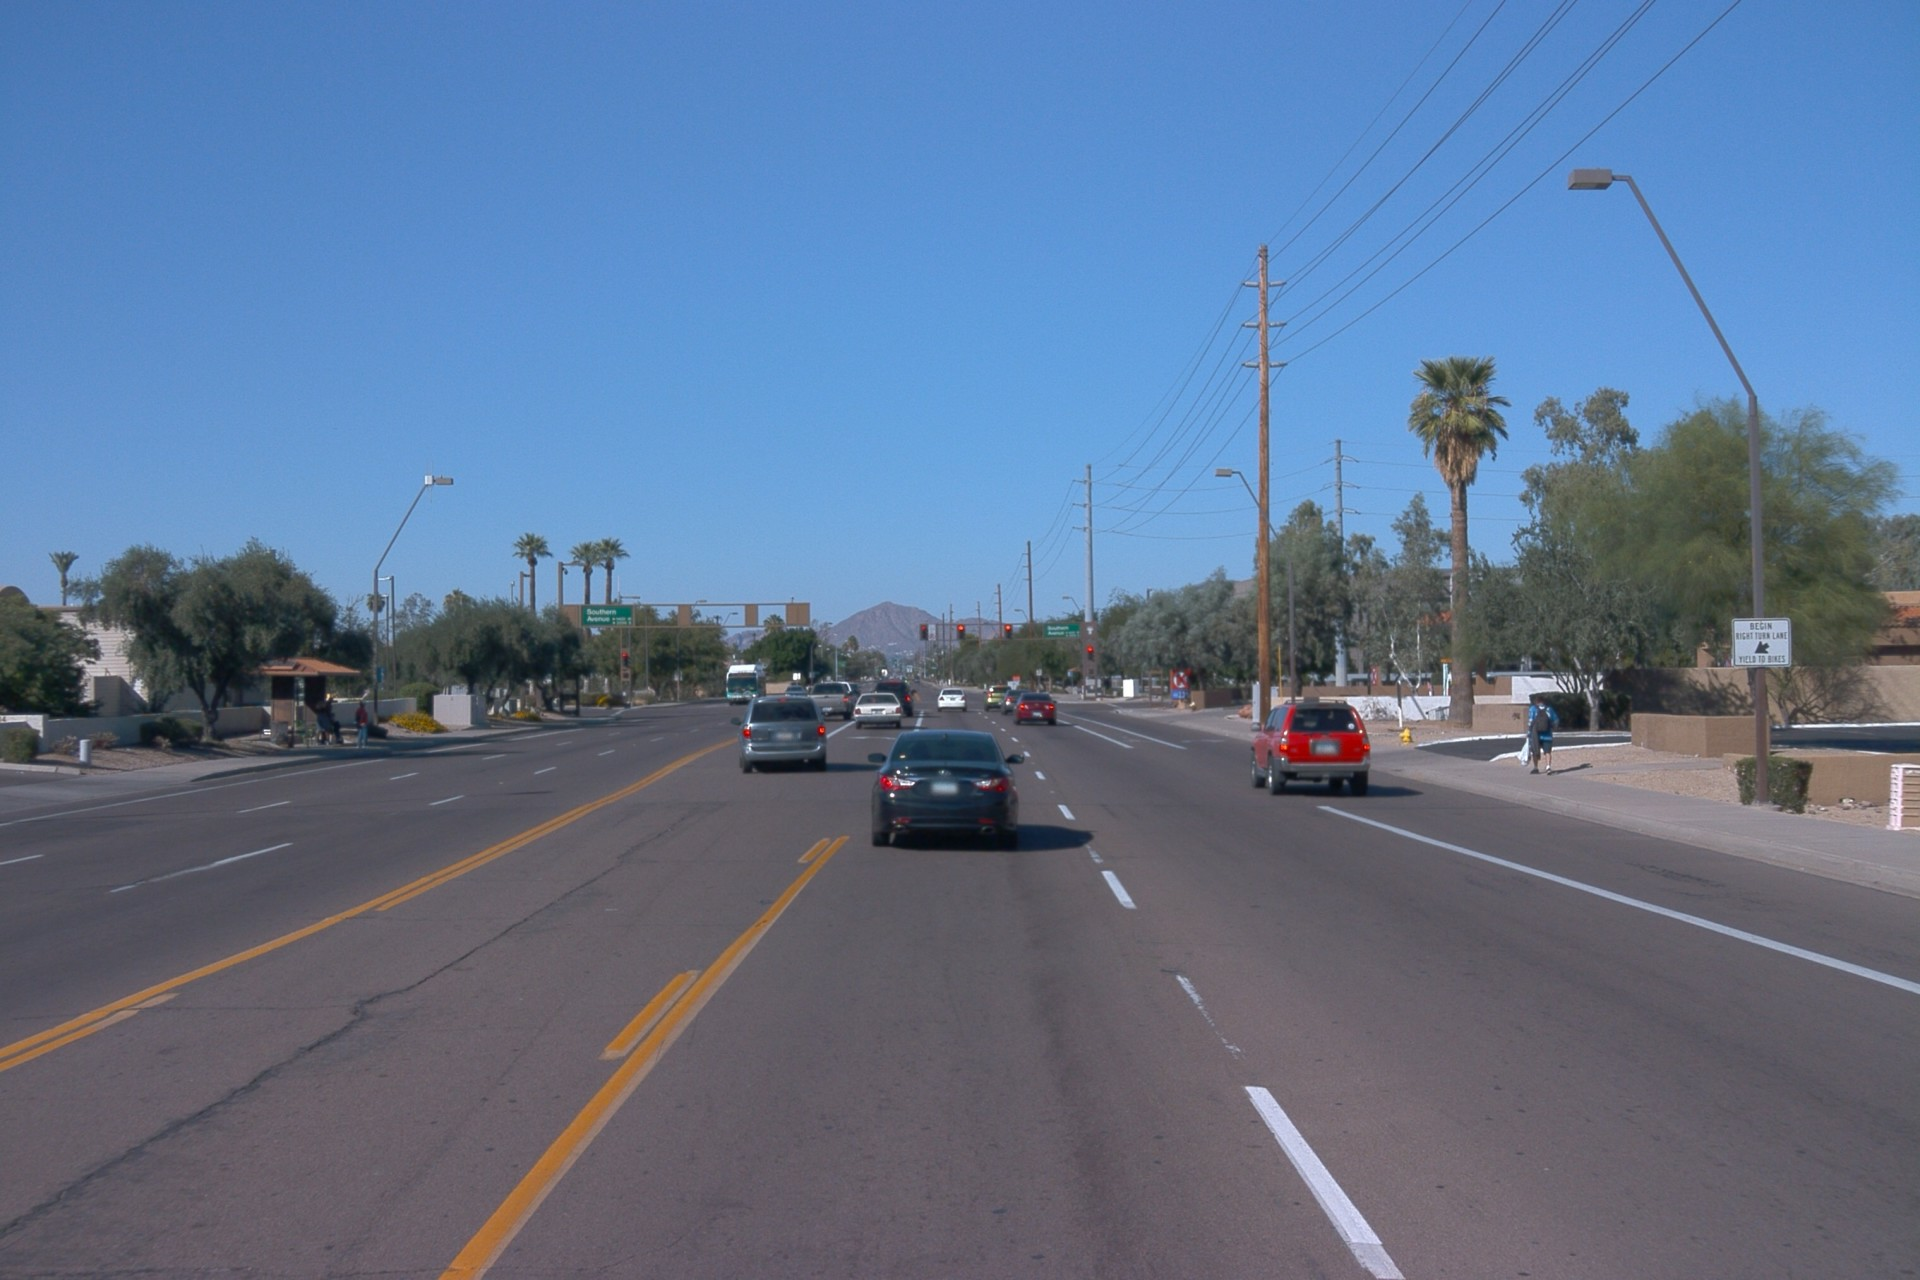
\includegraphics[width=.44\columnwidth, trim={0cm 0cm 0cm 0cm},clip]{fig/optim_supplement/scene50/initial_guess_50_10_waymo.png}&
% 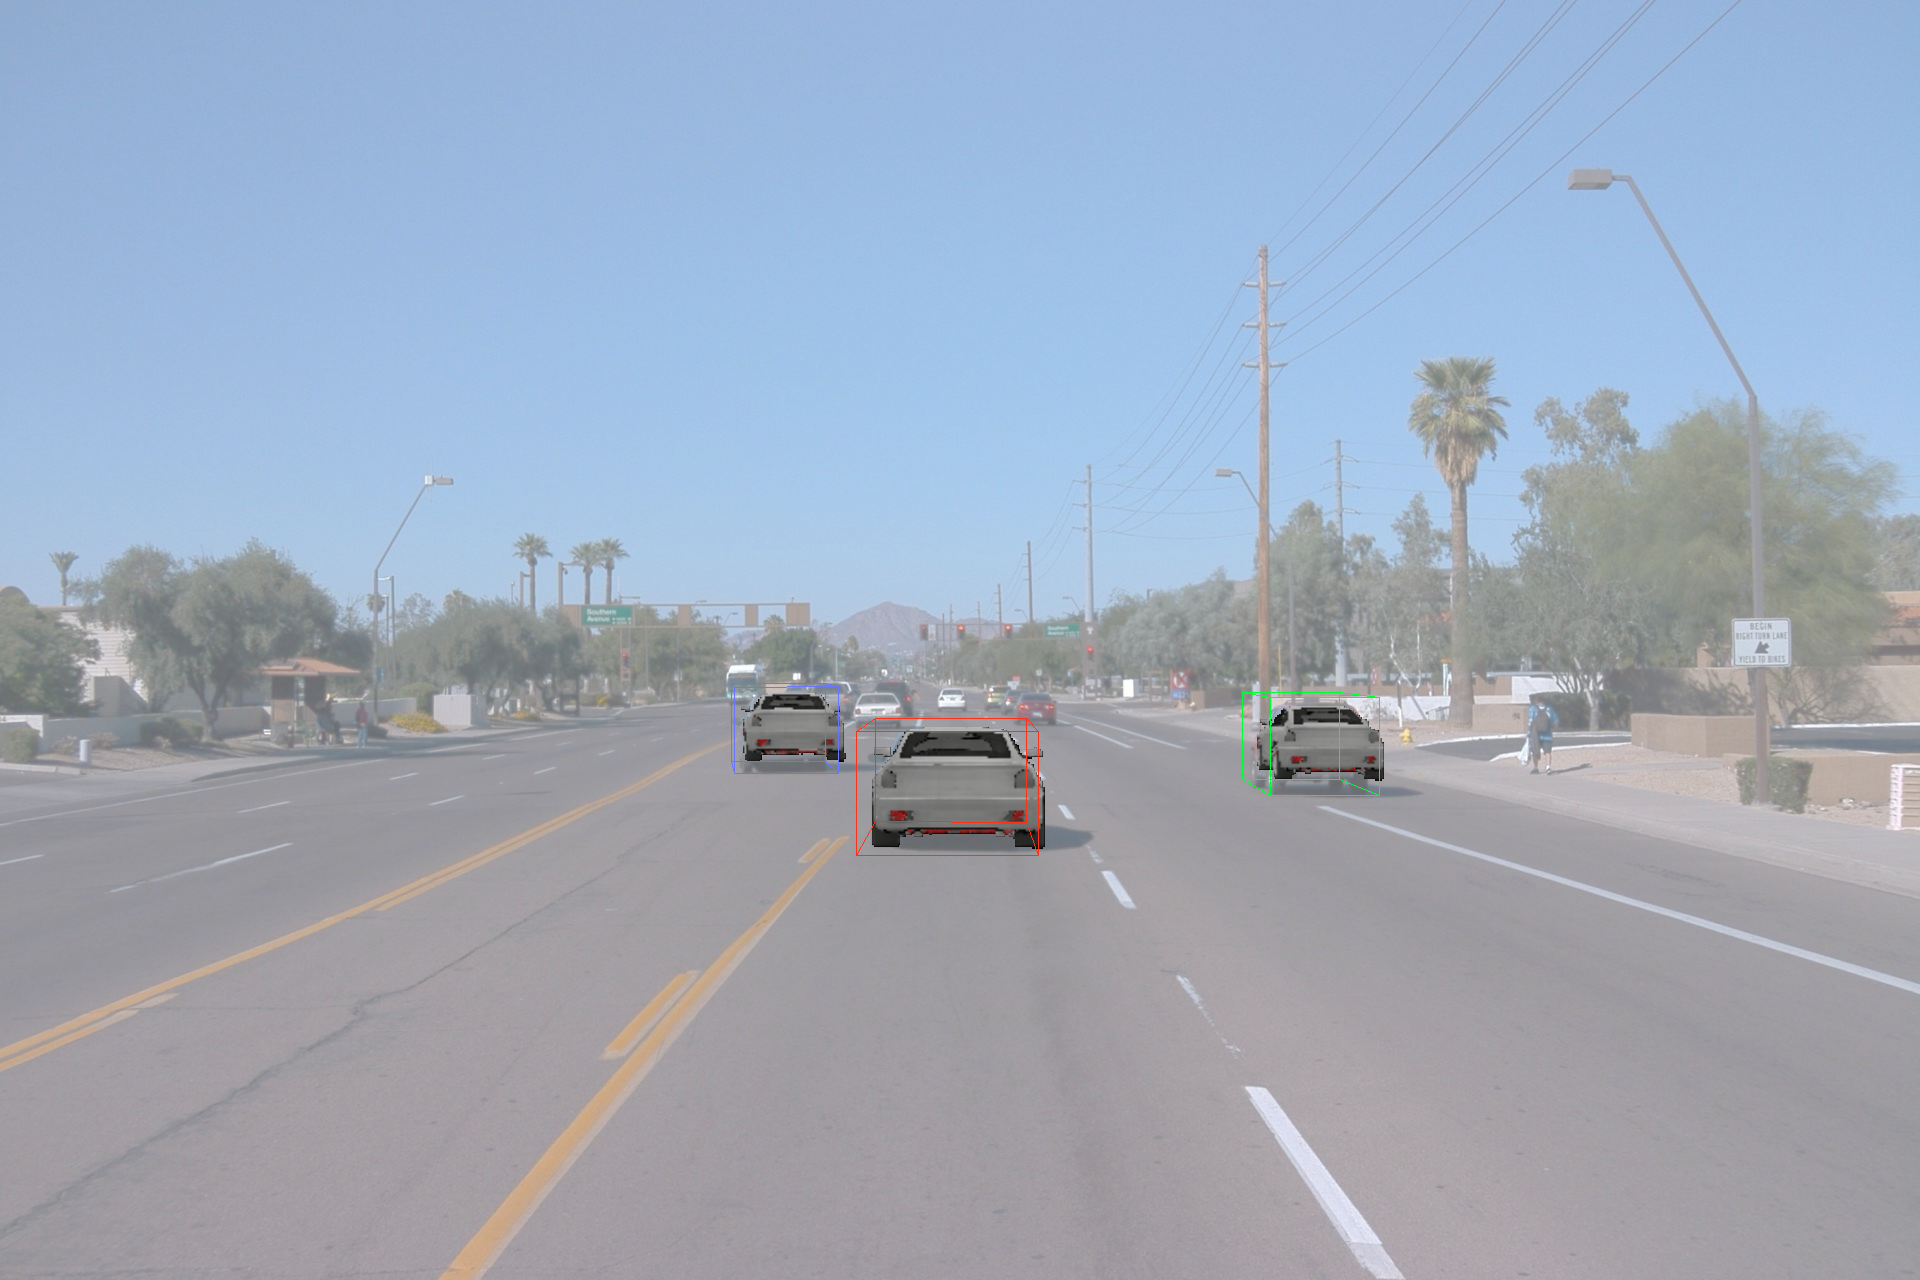
\includegraphics[width=.44\columnwidth, trim={0cm 0cm 0cm 0cm},clip]{fig/optim_supplement/scene50/init_guess-50.png}&
% 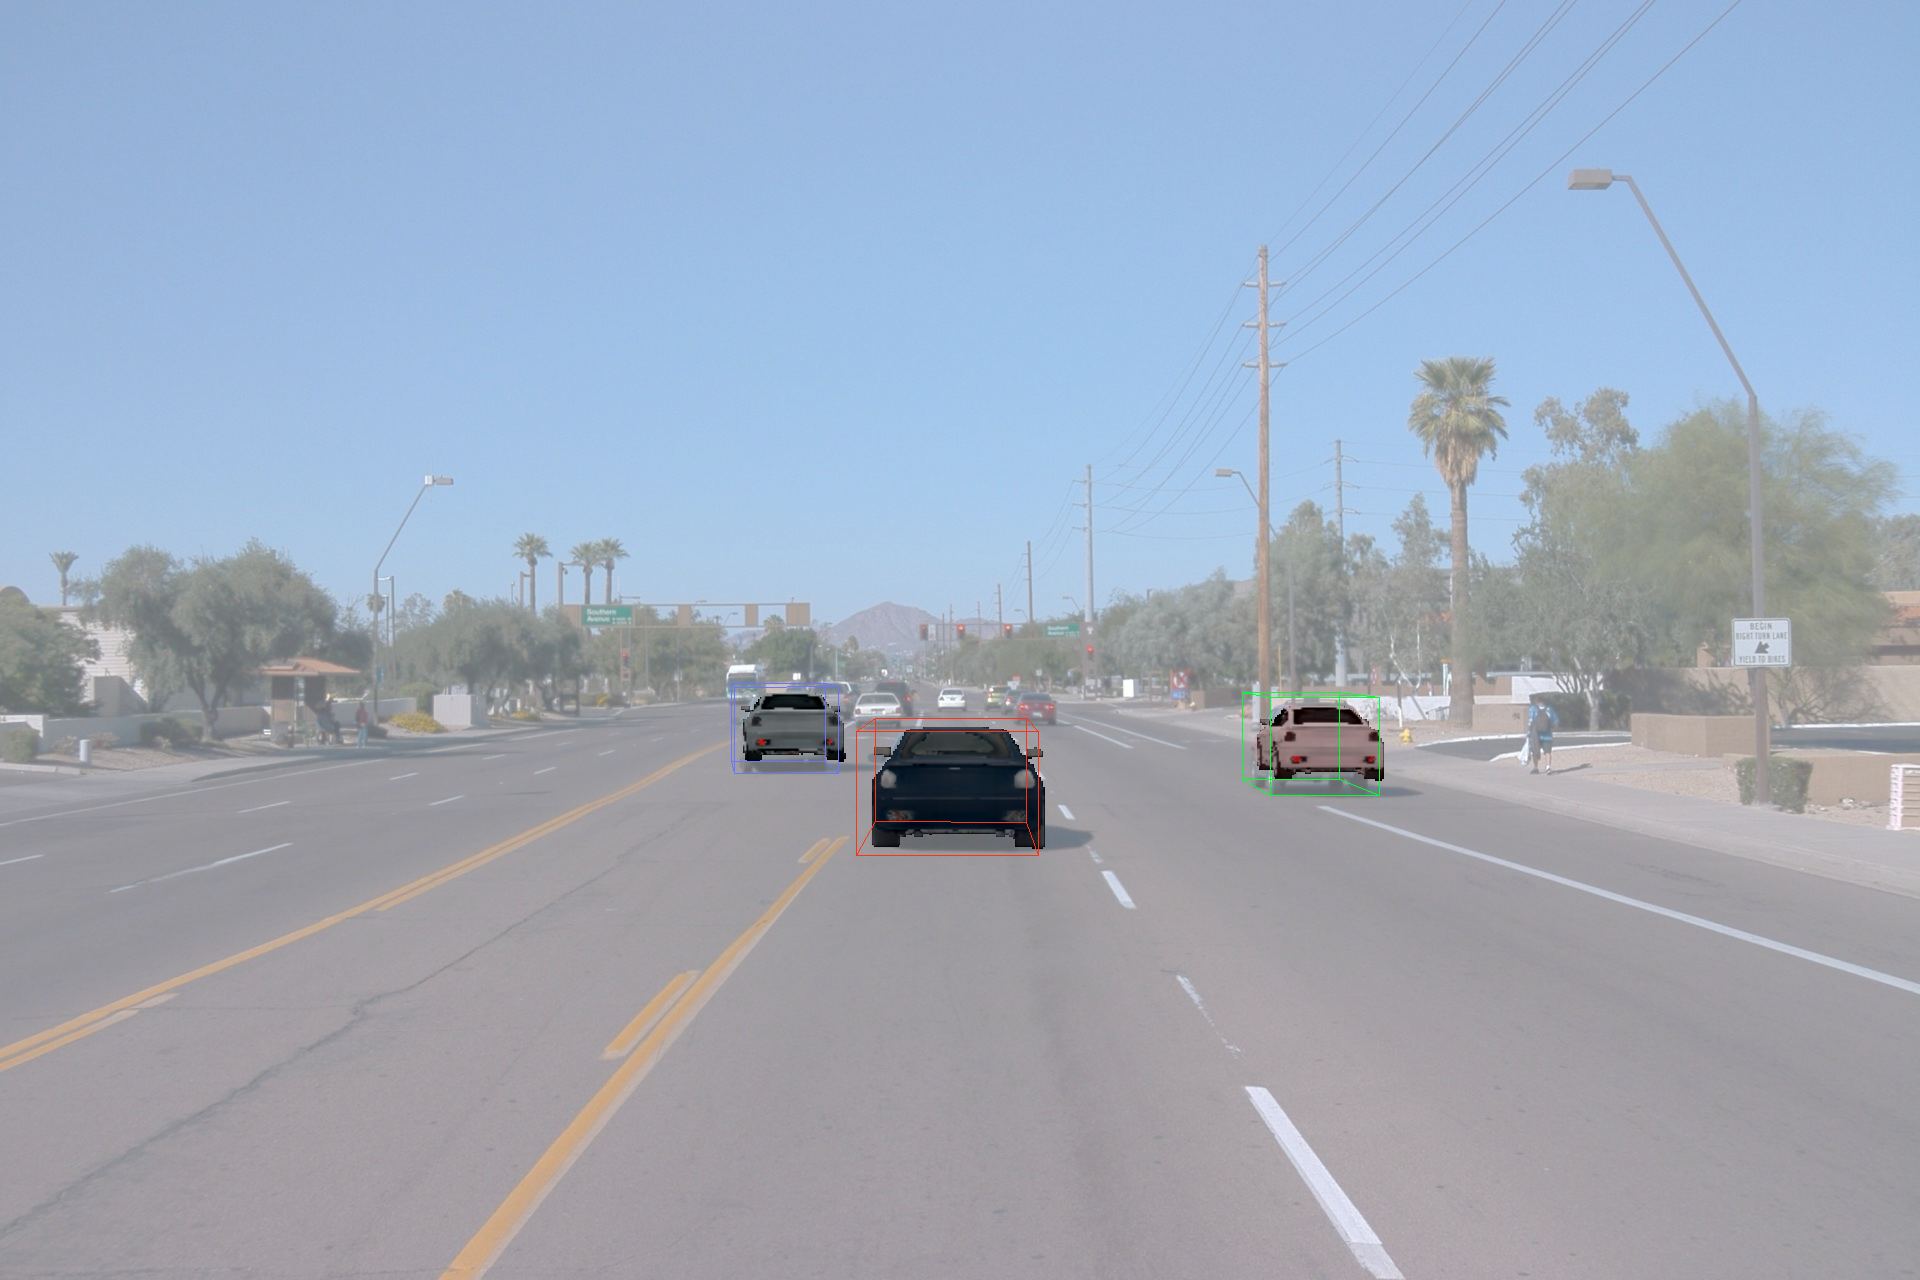
\includegraphics[width=.44\columnwidth, trim={0cm 0cm 0cm 0cm},clip]{fig/optim_supplement/scene50/tex_50_10.png}&
% 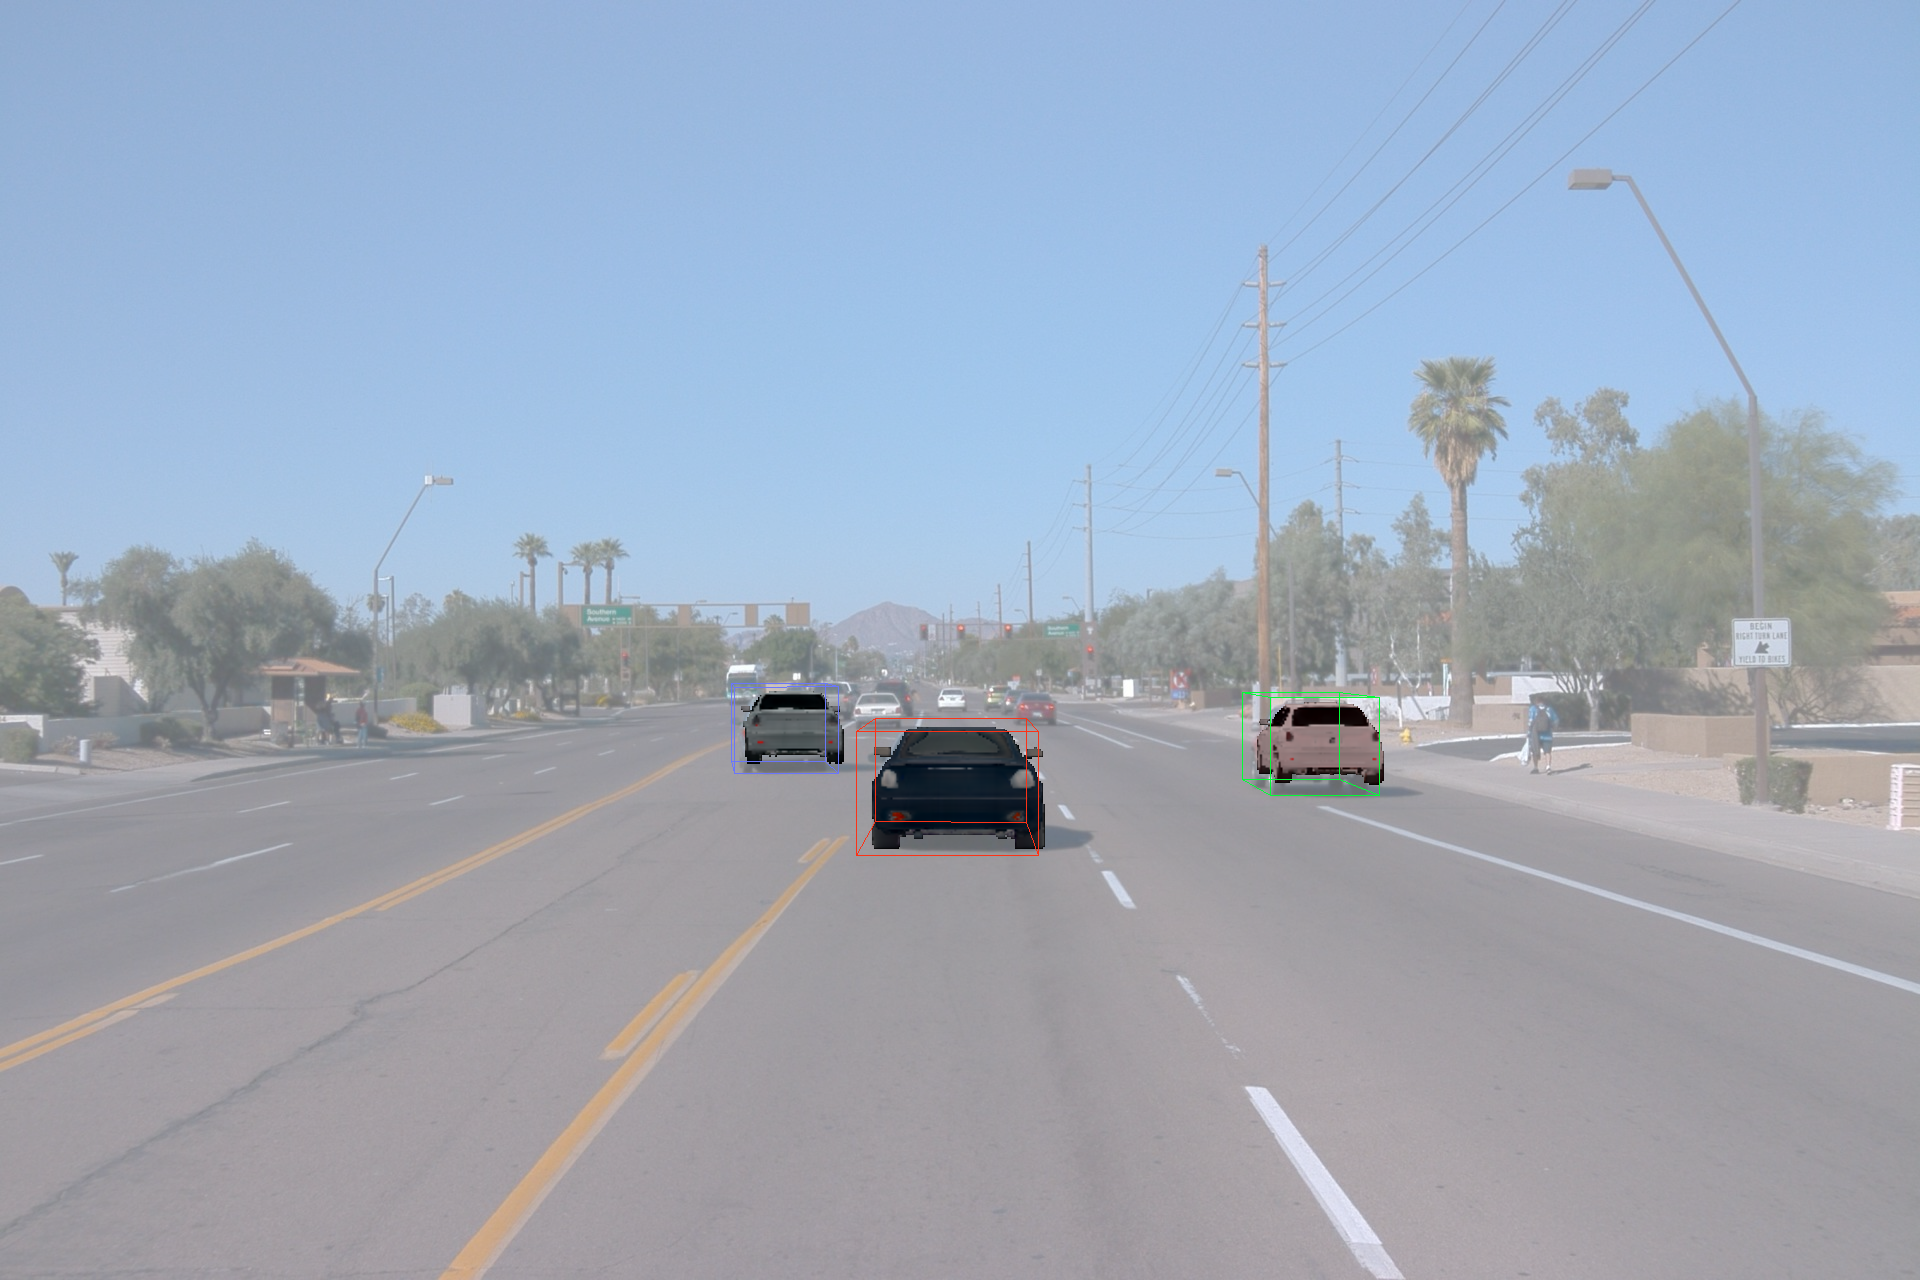
\includegraphics[width=.44\columnwidth, trim={0cm 0cm 0cm 0cm},clip]{fig/optim_supplement/scene50/4_50_10.png}&
% 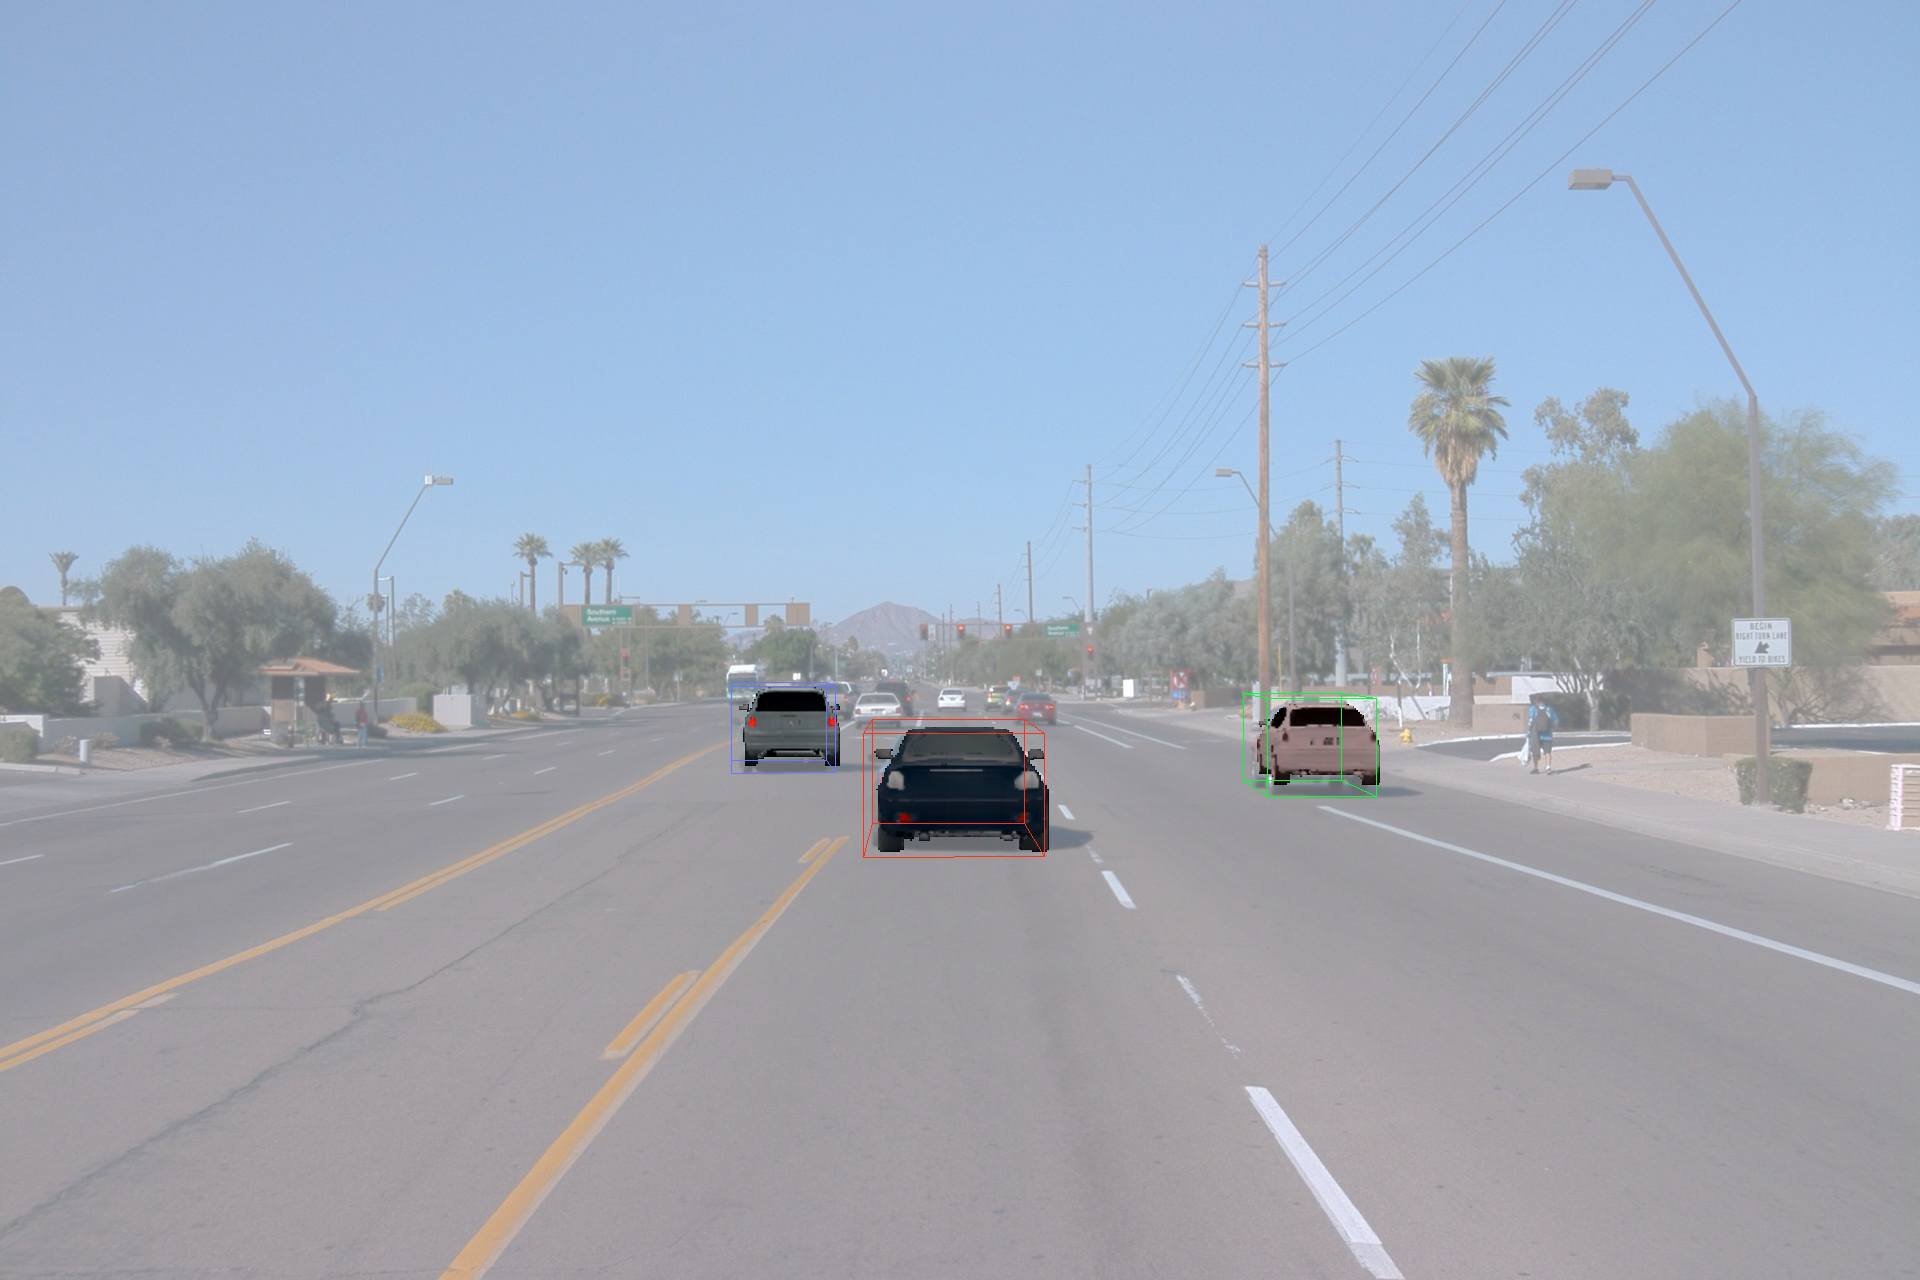
\includegraphics[width=.44\columnwidth, trim={0cm 0cm 0cm 0cm},clip]{fig/optim_supplement/scene50/5_50_10.png} \\

% 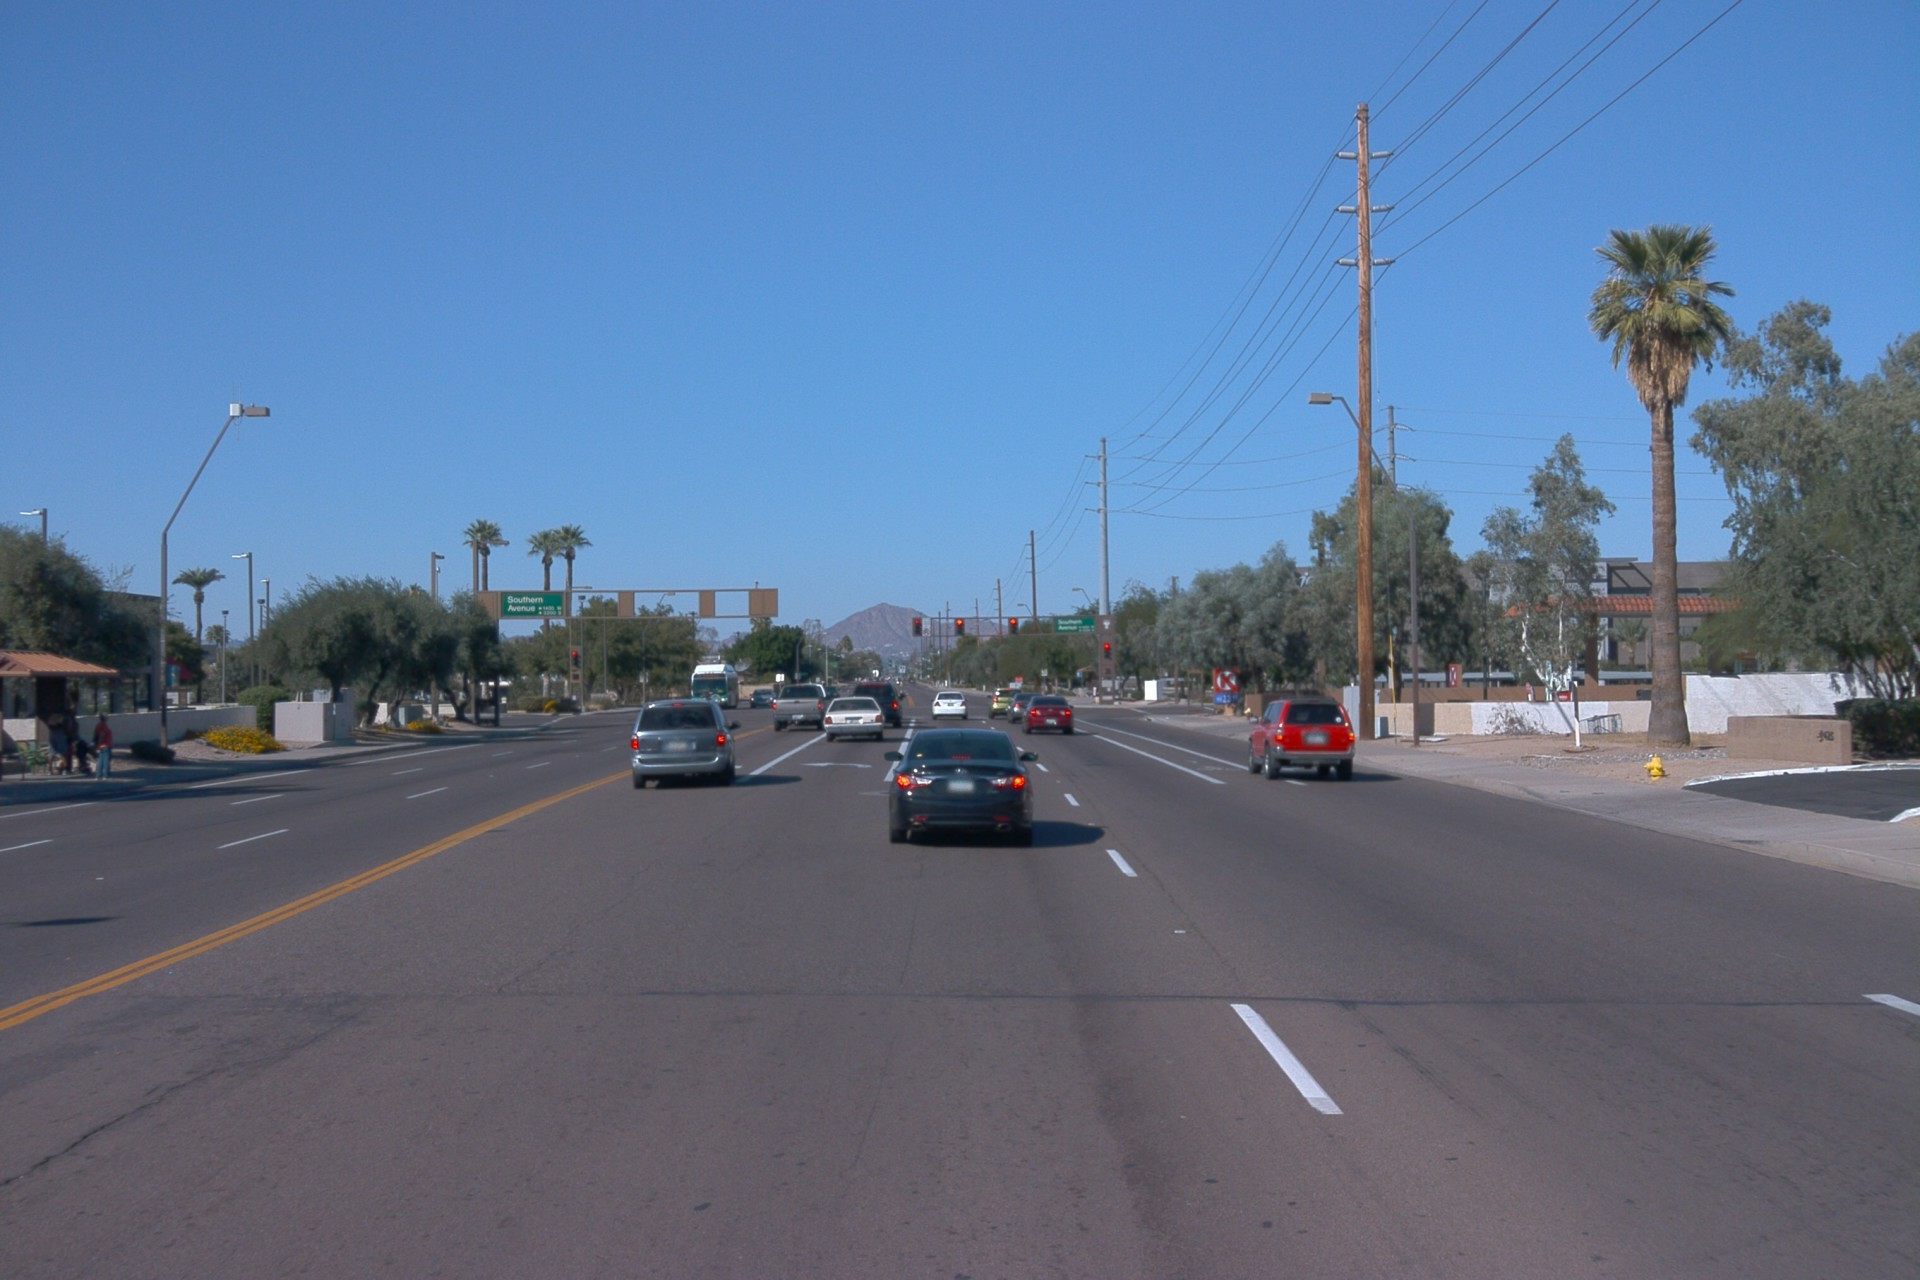
\includegraphics[width=.44\columnwidth, trim={0cm 0cm 0cm 0cm},clip]{fig/optim_supplement/scene50_26/50_26_gt.png}&
% 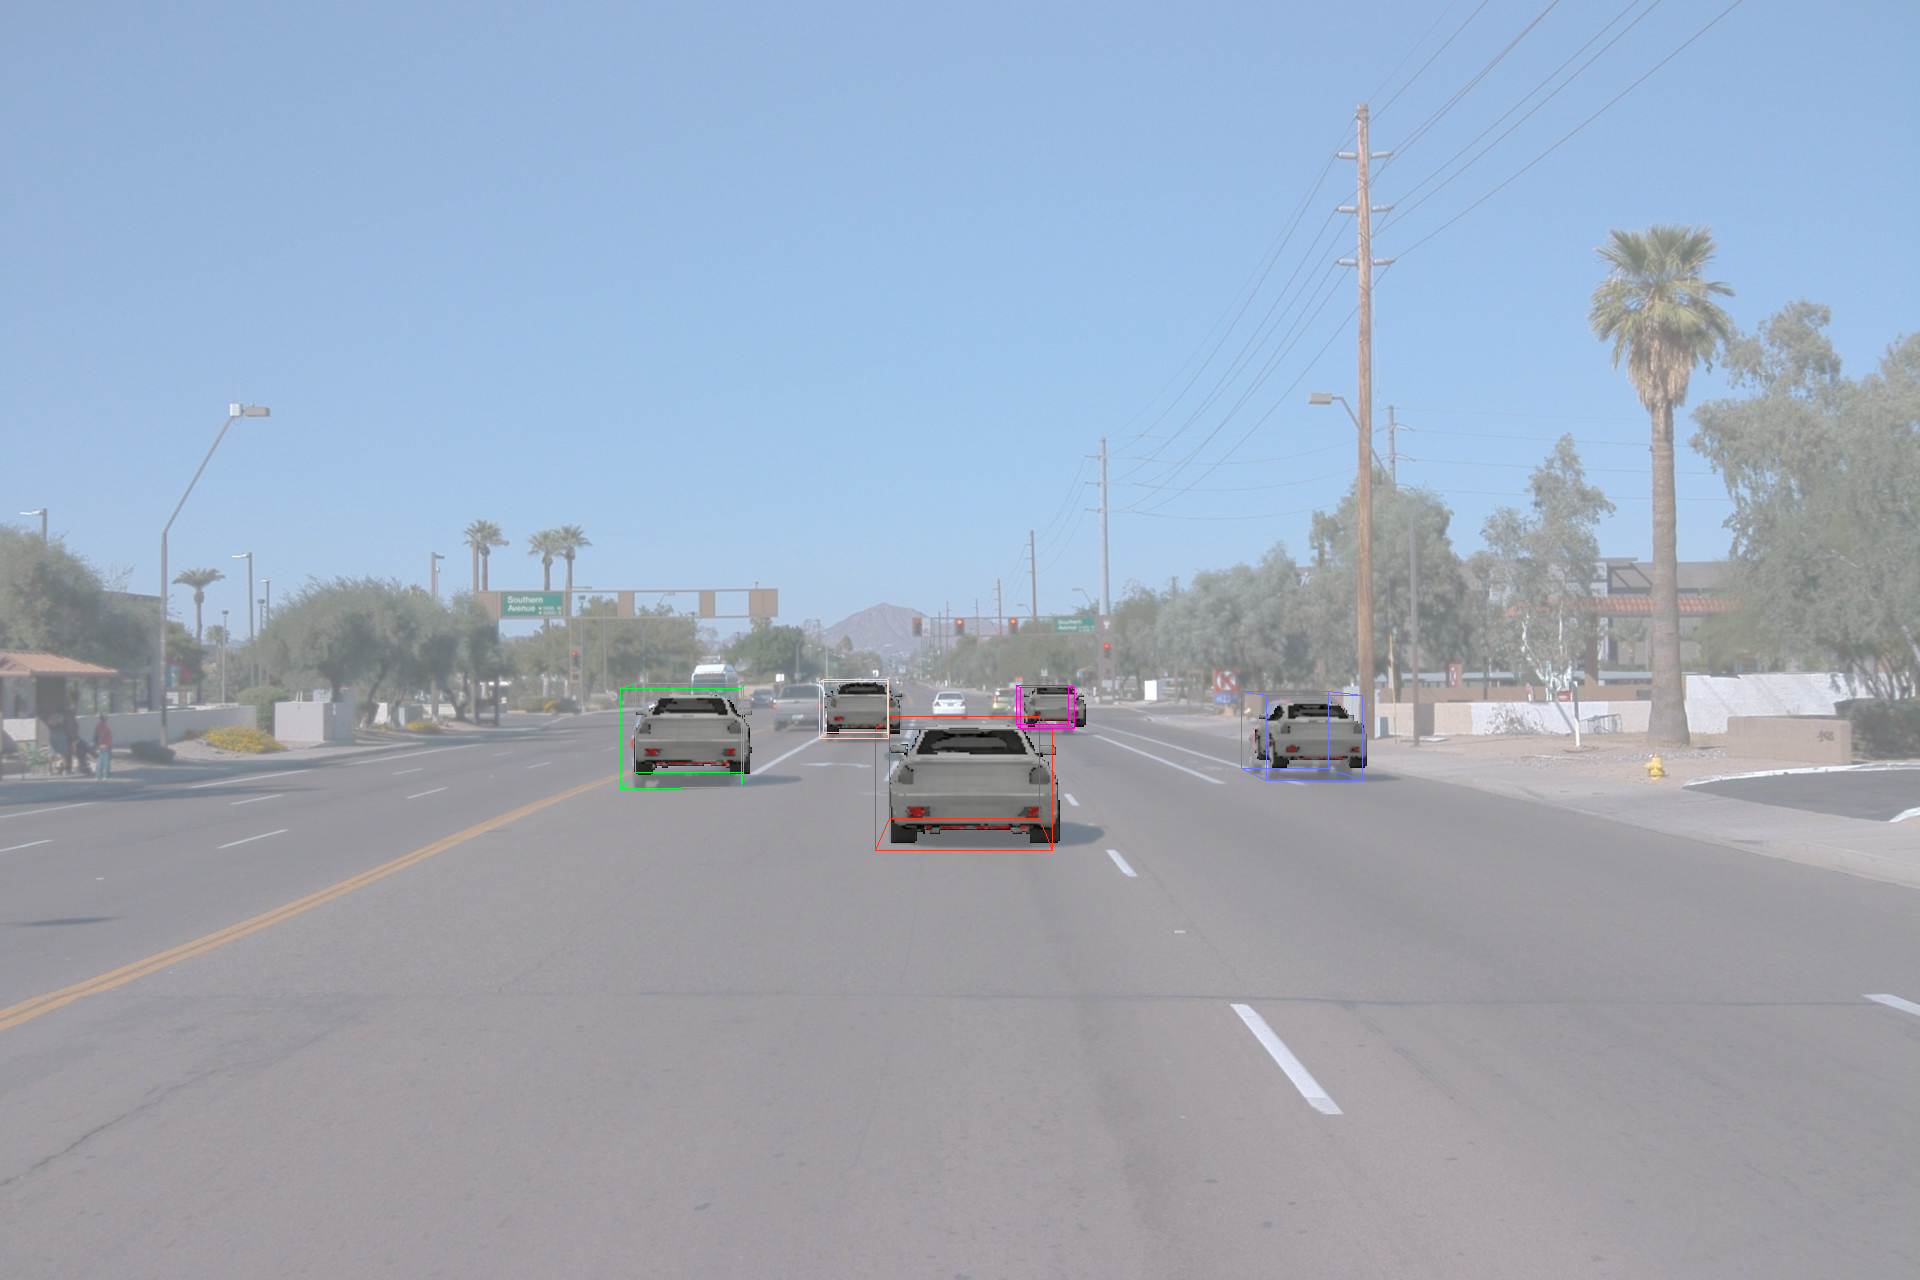
\includegraphics[width=.44\columnwidth, trim={0cm 0cm 0cm 0cm},clip]{fig/optim_supplement/scene50_26/50_26_0.png}&
% 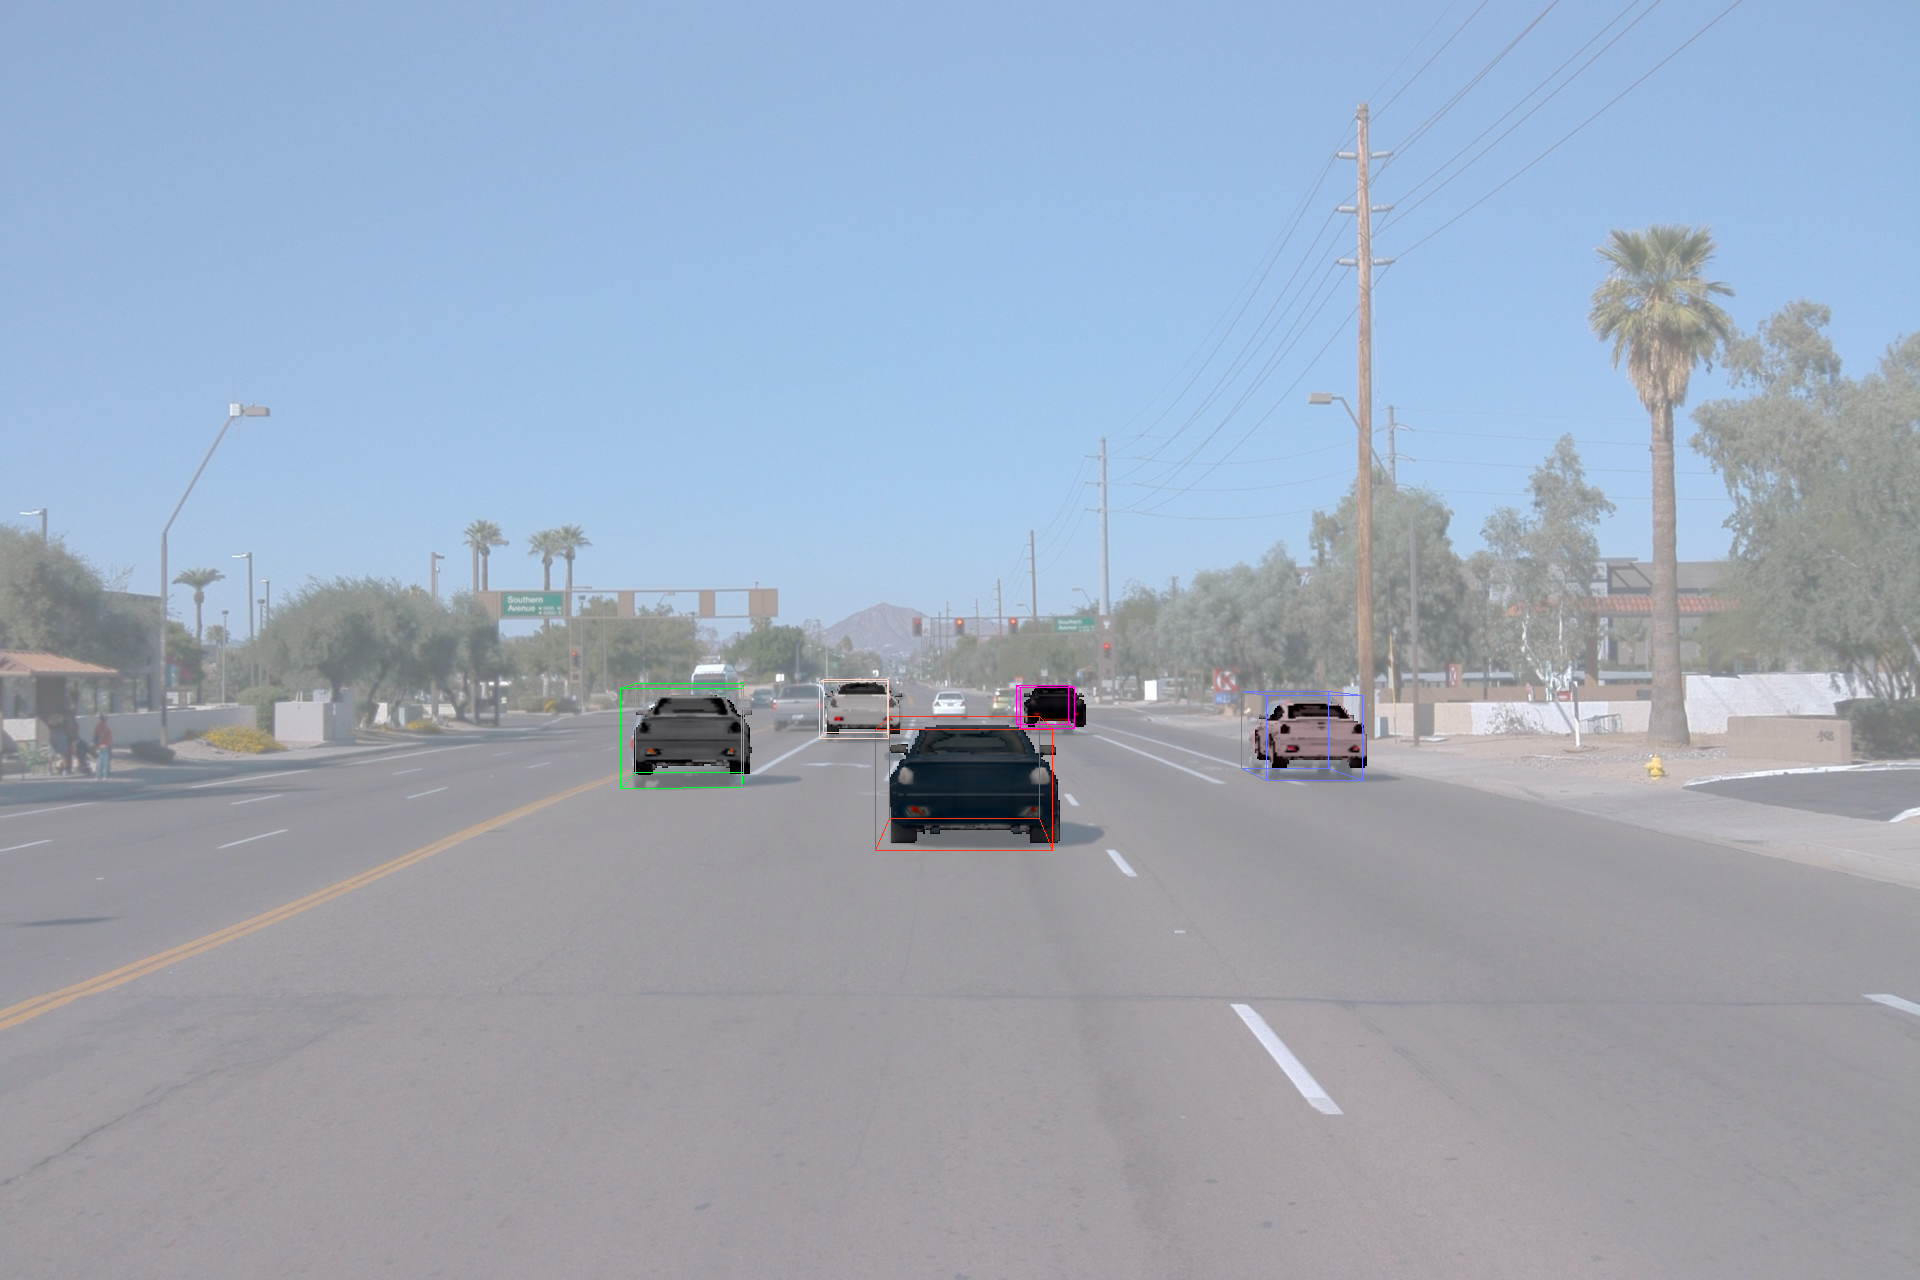
\includegraphics[width=.44\columnwidth, trim={0cm 0cm 0cm 0cm},clip]{fig/optim_supplement/scene50_26/50_26_3.png}&
% 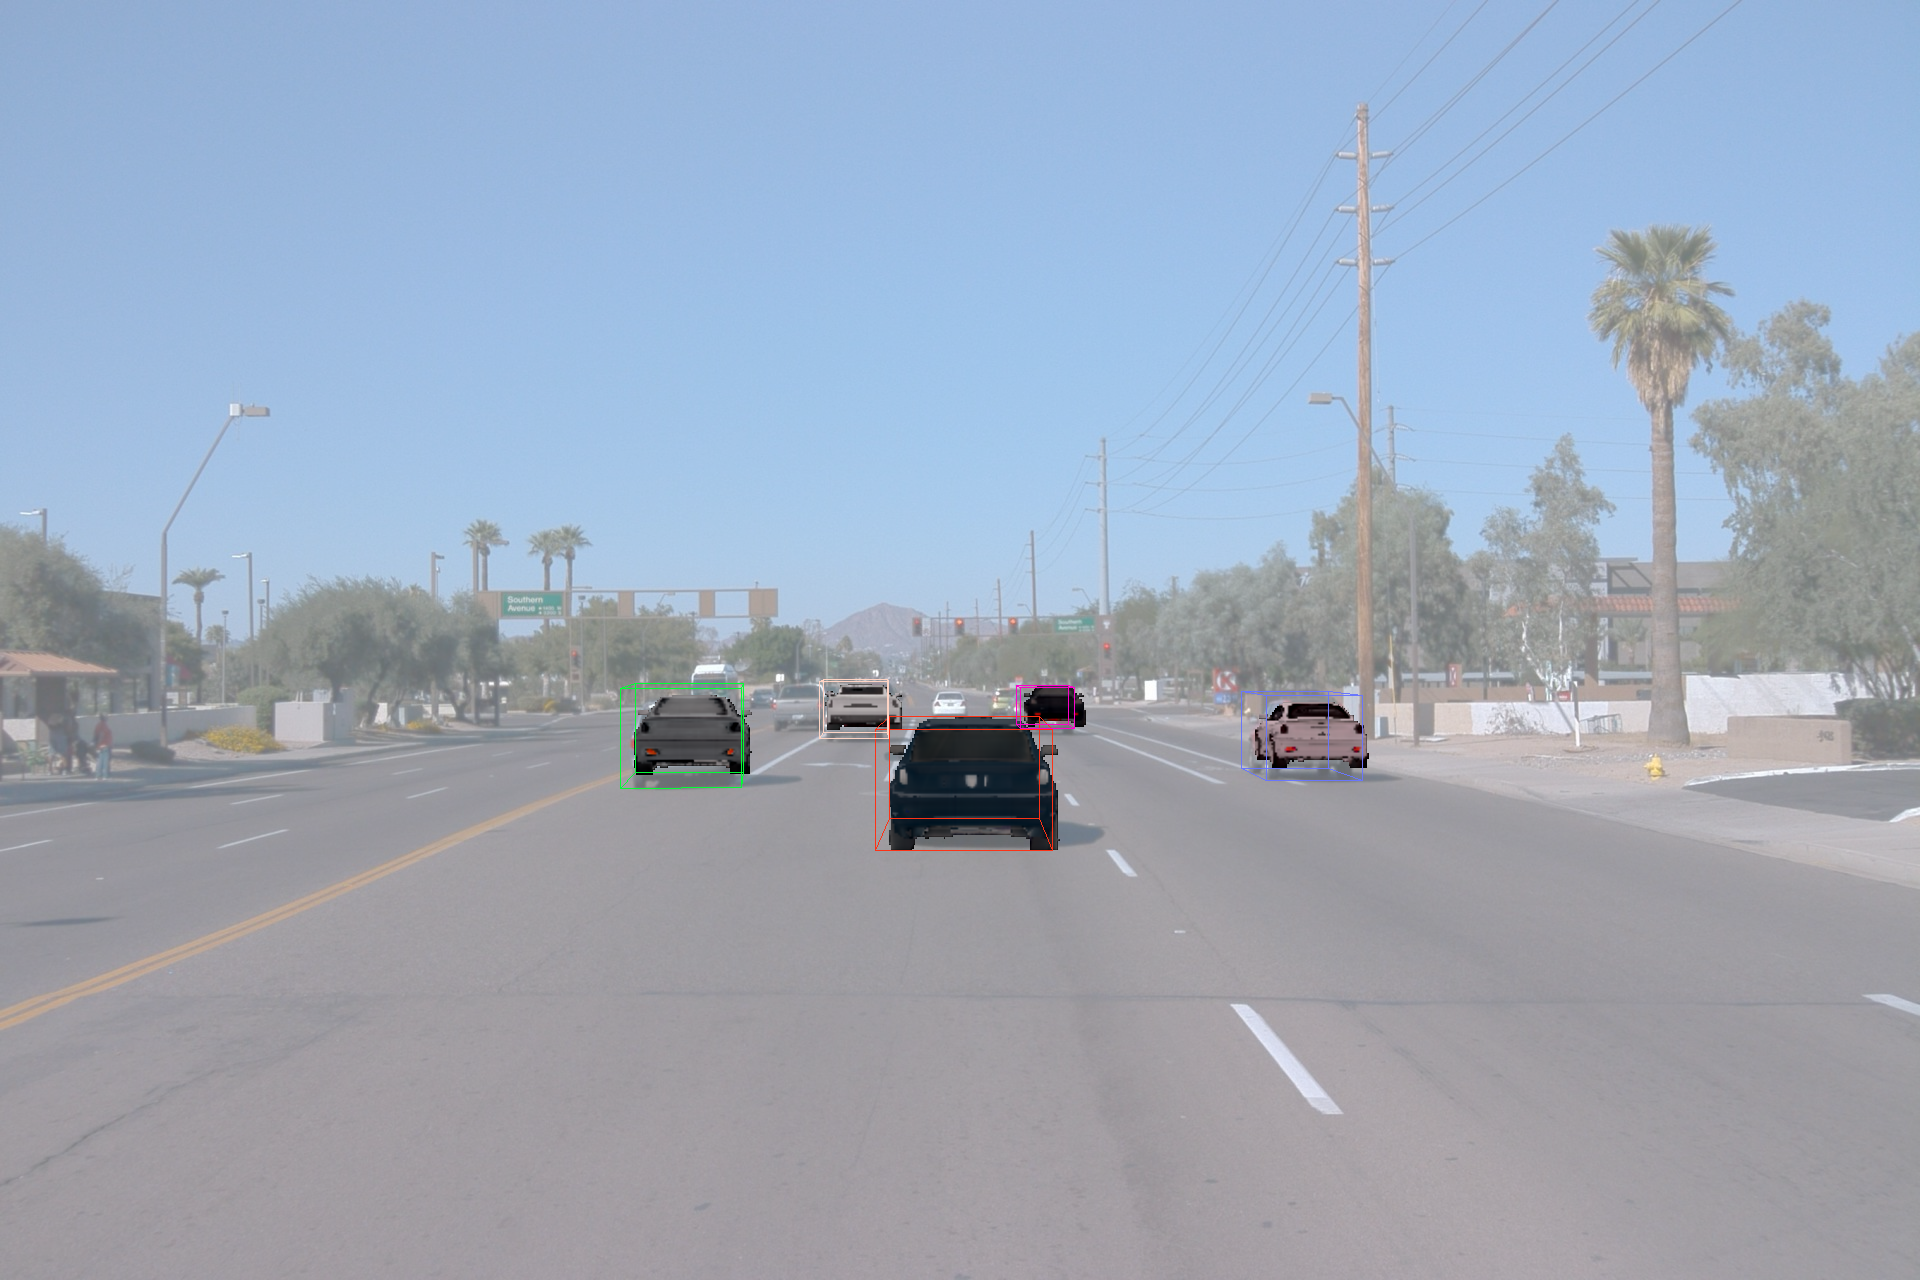
\includegraphics[width=.44\columnwidth, trim={0cm 0cm 0cm 0cm},clip]{fig/optim_supplement/scene50_26/50_26_4.png}&
% 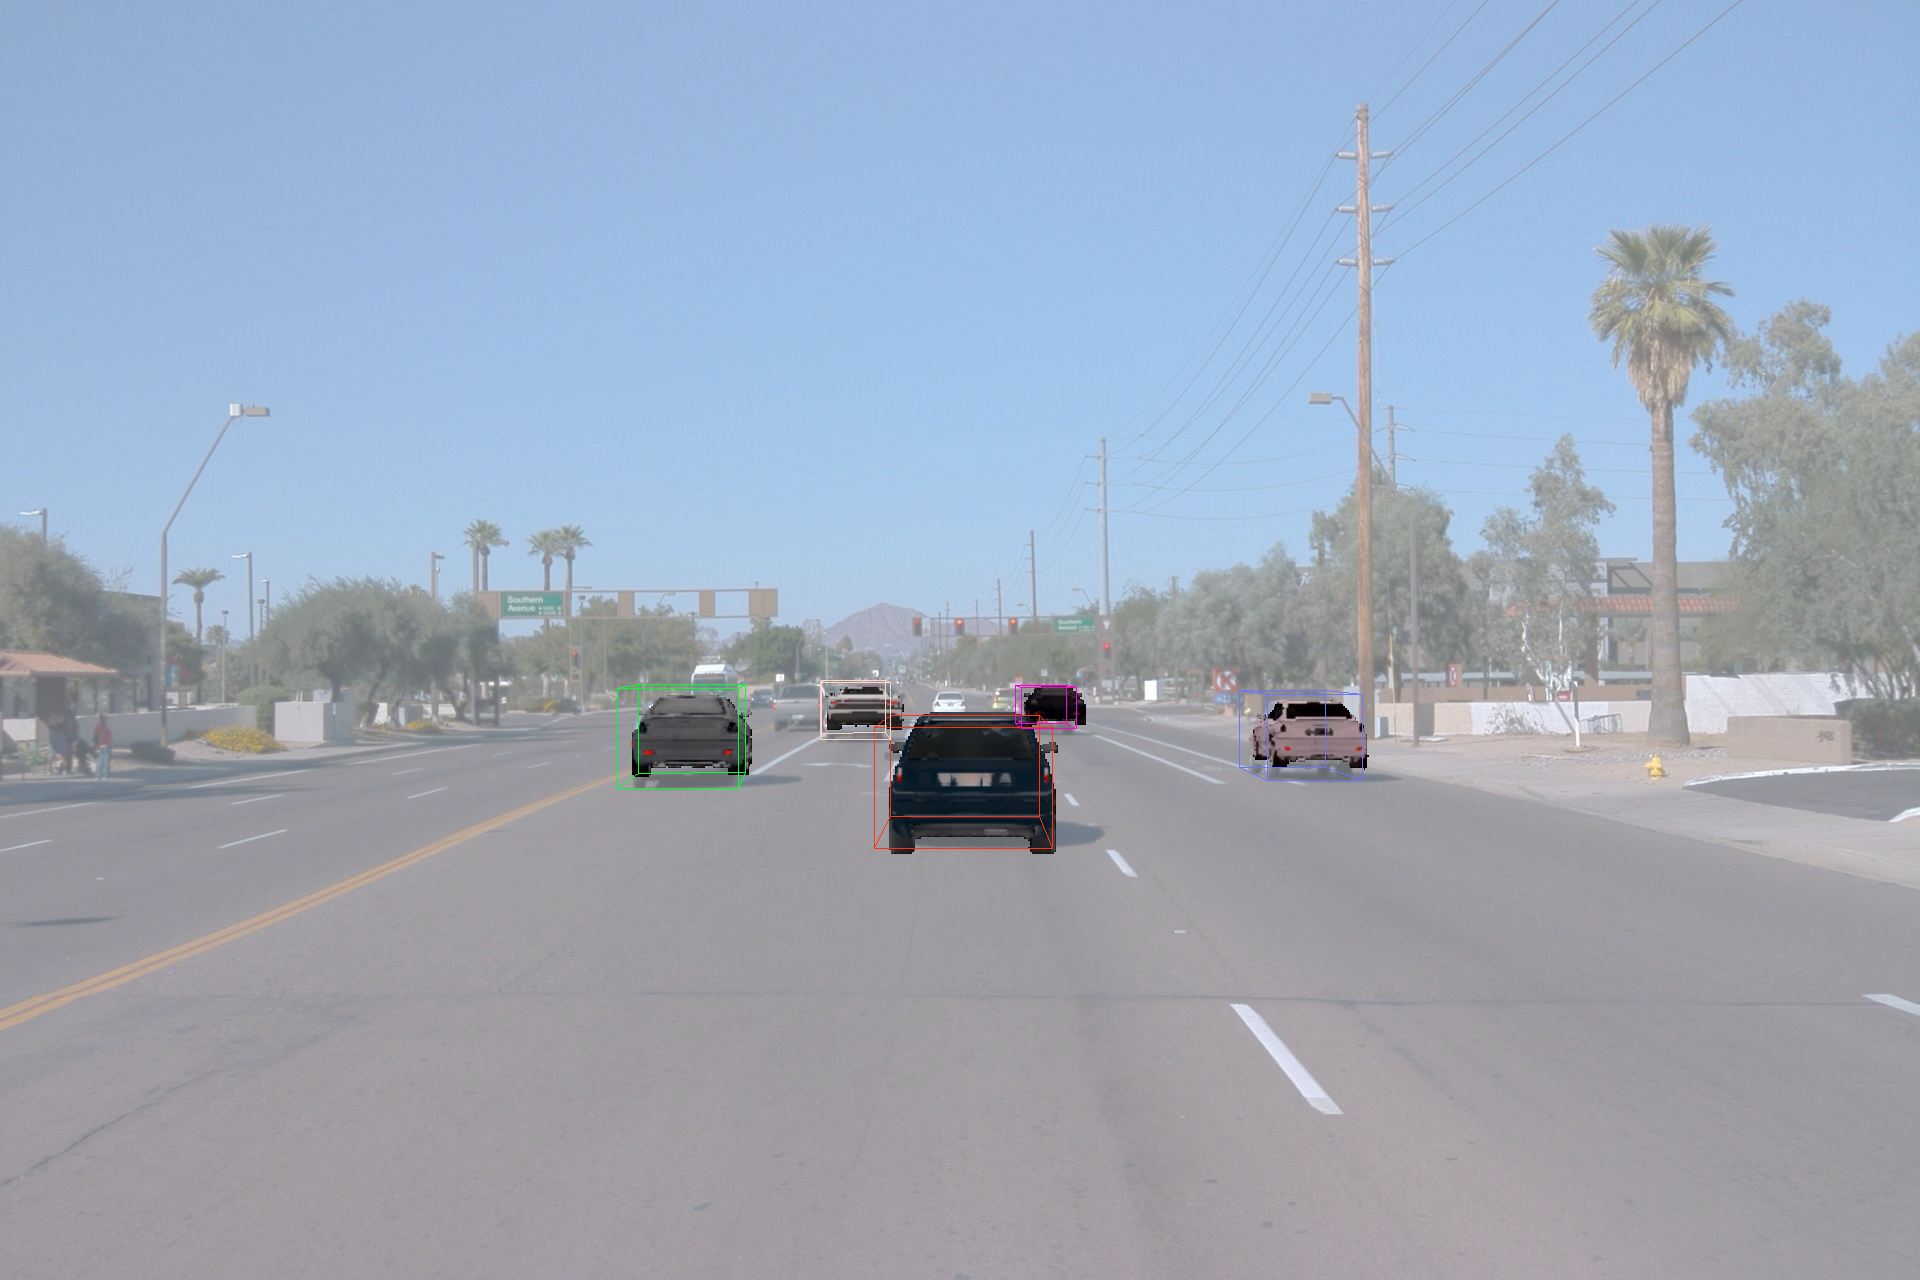
\includegraphics[width=.44\columnwidth, trim={0cm 0cm 0cm 0cm},clip]{fig/optim_supplement/scene50_26/50_26_5.png} \\

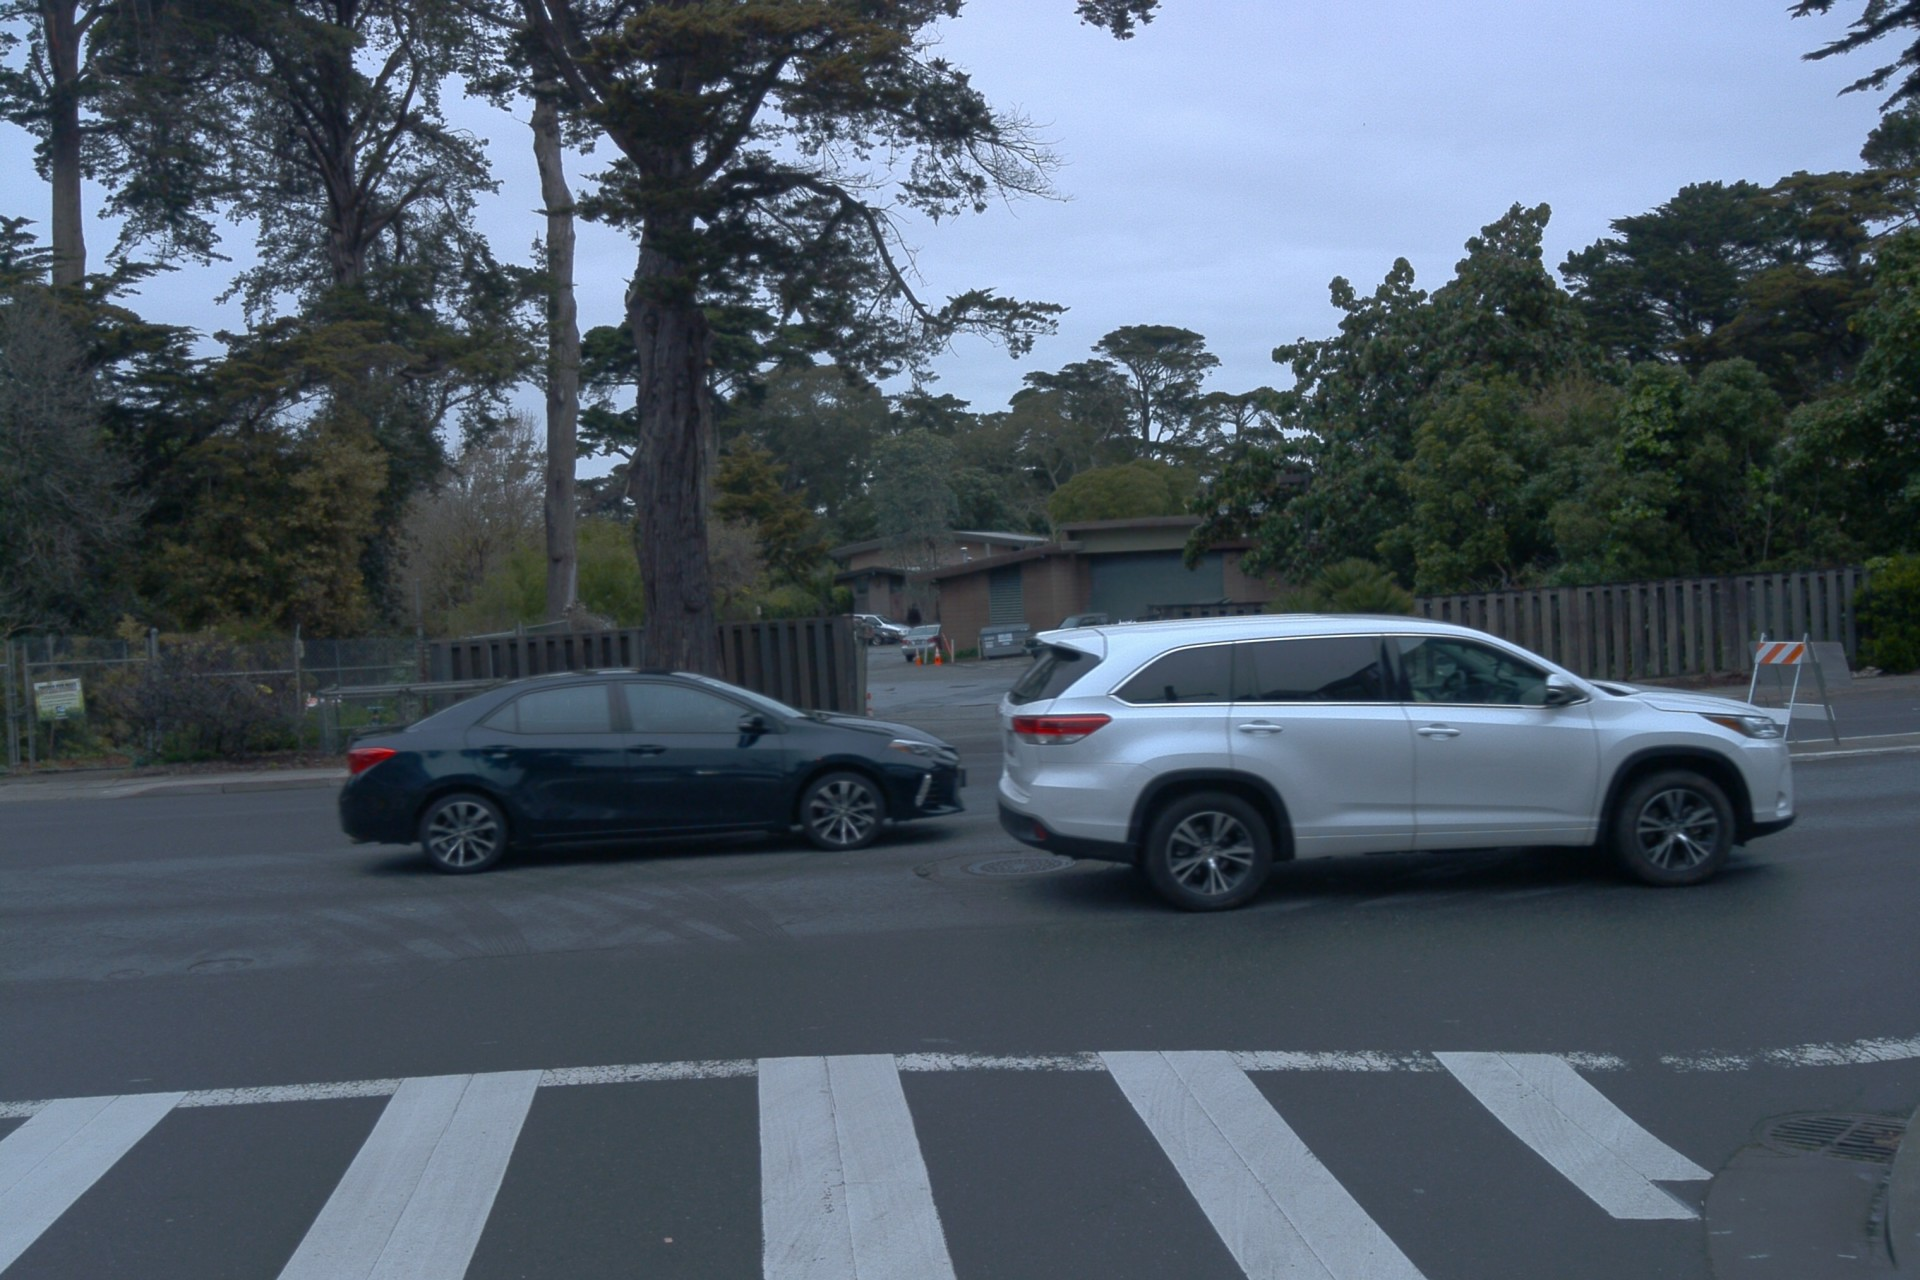
\includegraphics[width=.44\columnwidth, trim={0cm 0cm 0cm 0cm},clip]{fig/optim_supplement/scene11_104/gt_img.png}&
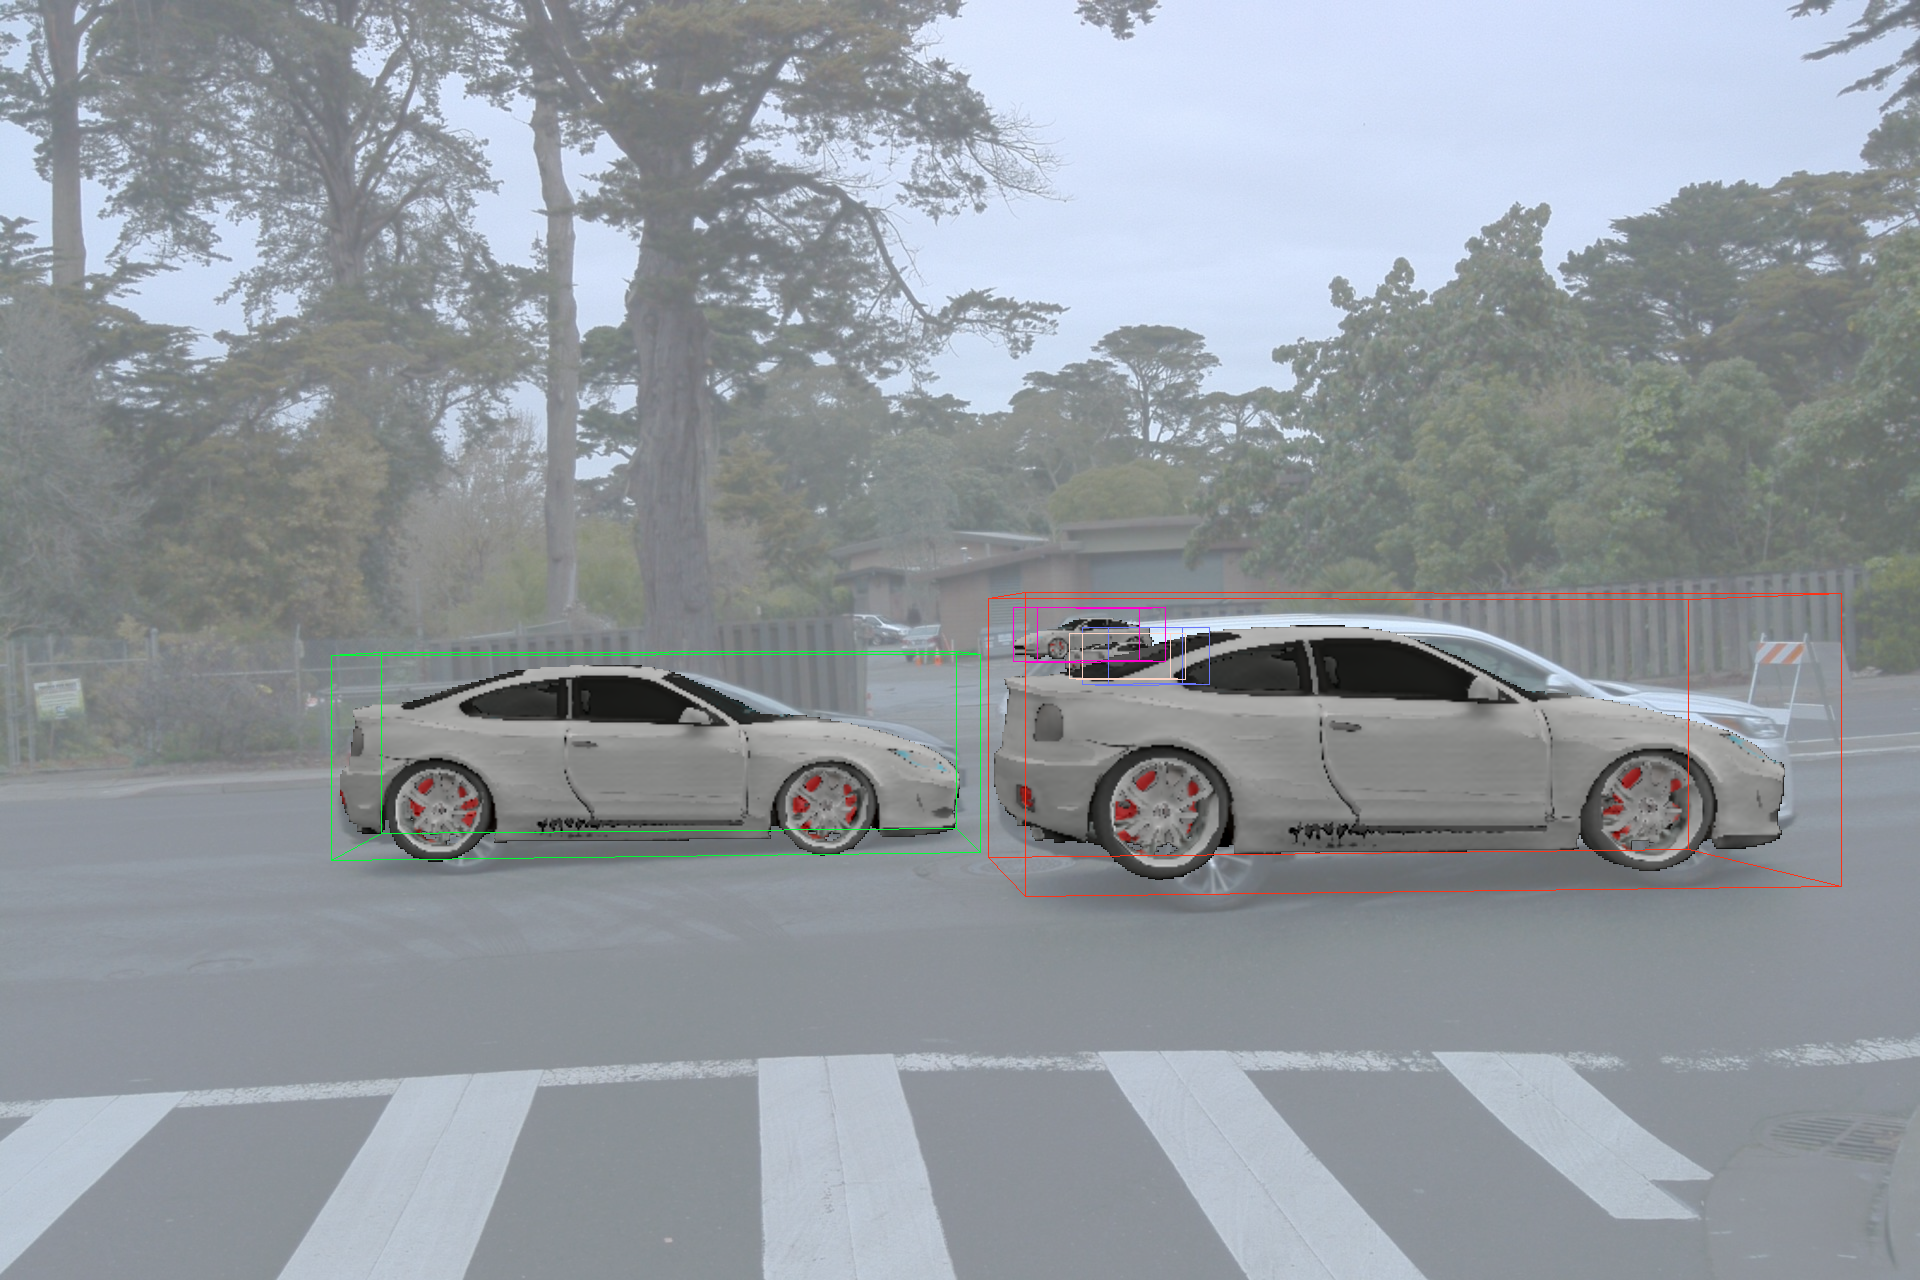
\includegraphics[width=.44\columnwidth, trim={0cm 0cm 0cm 0cm},clip]{fig/optim_supplement/scene11_104/init.png}&
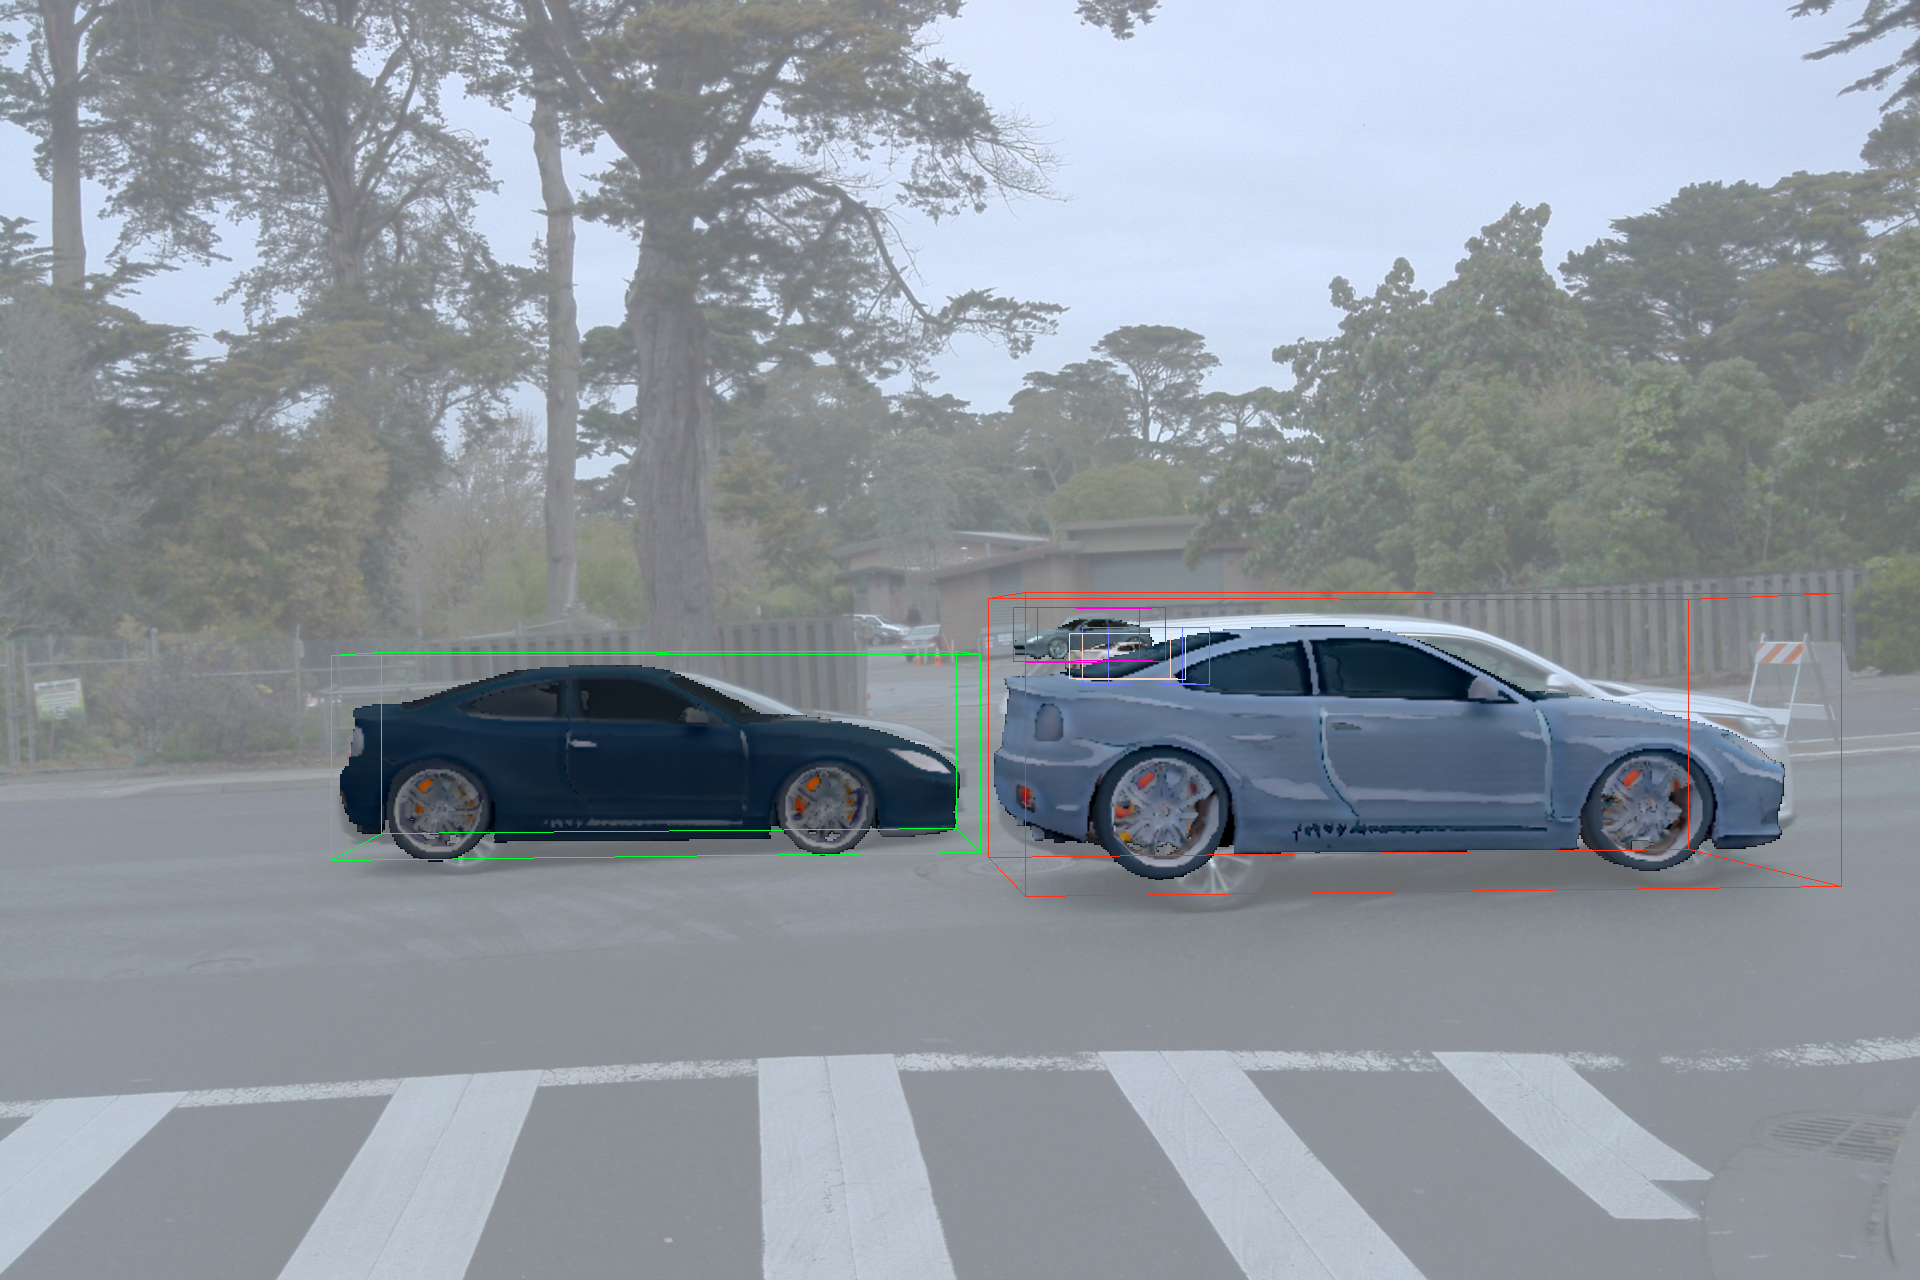
\includegraphics[width=.44\columnwidth, trim={0cm 0cm 0cm 0cm},clip]{fig/optim_supplement/scene11_104/3.png}&
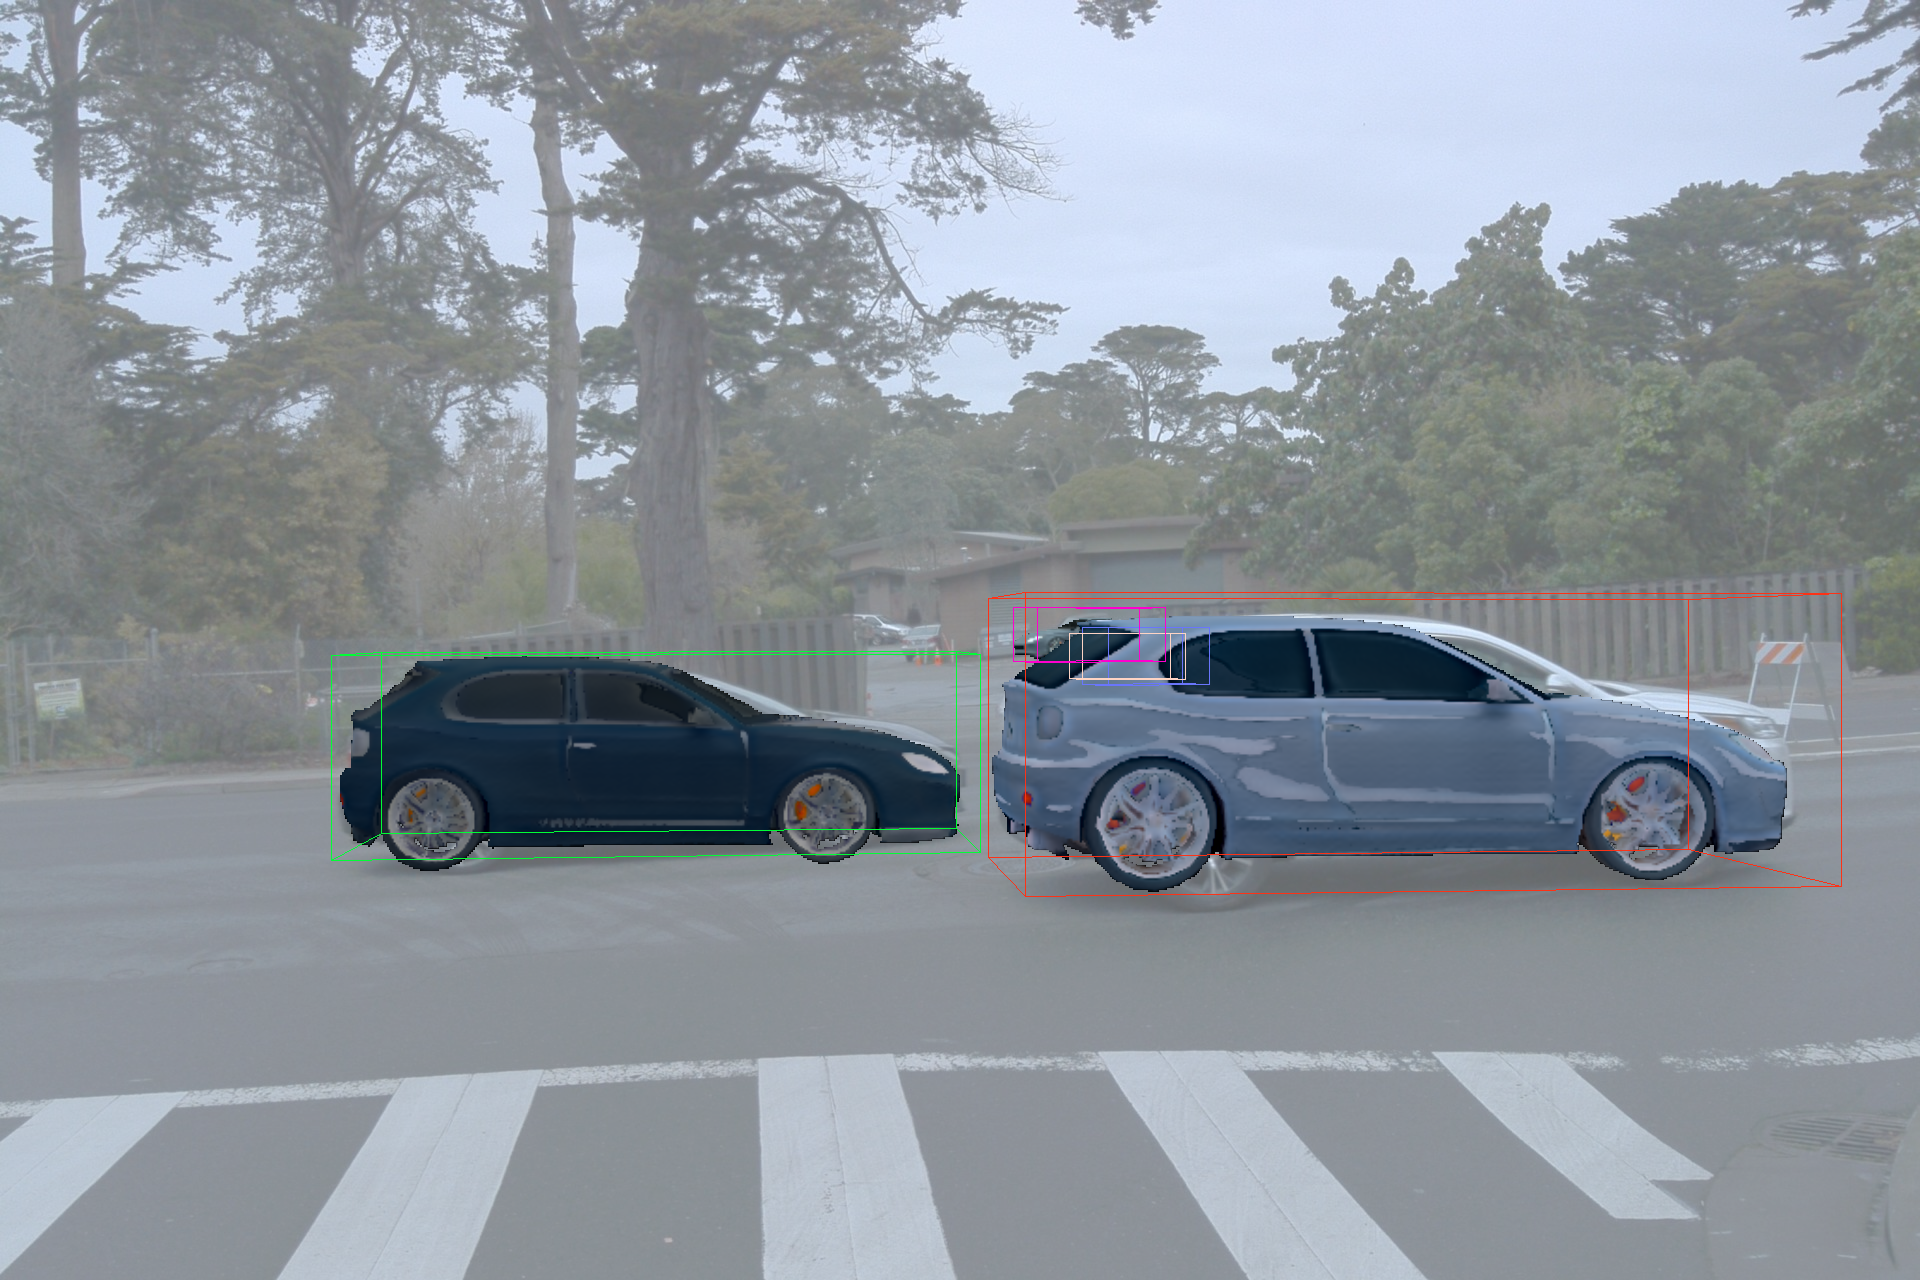
\includegraphics[width=.44\columnwidth, trim={0cm 0cm 0cm 0cm},clip]{fig/optim_supplement/scene11_104/4.png}&
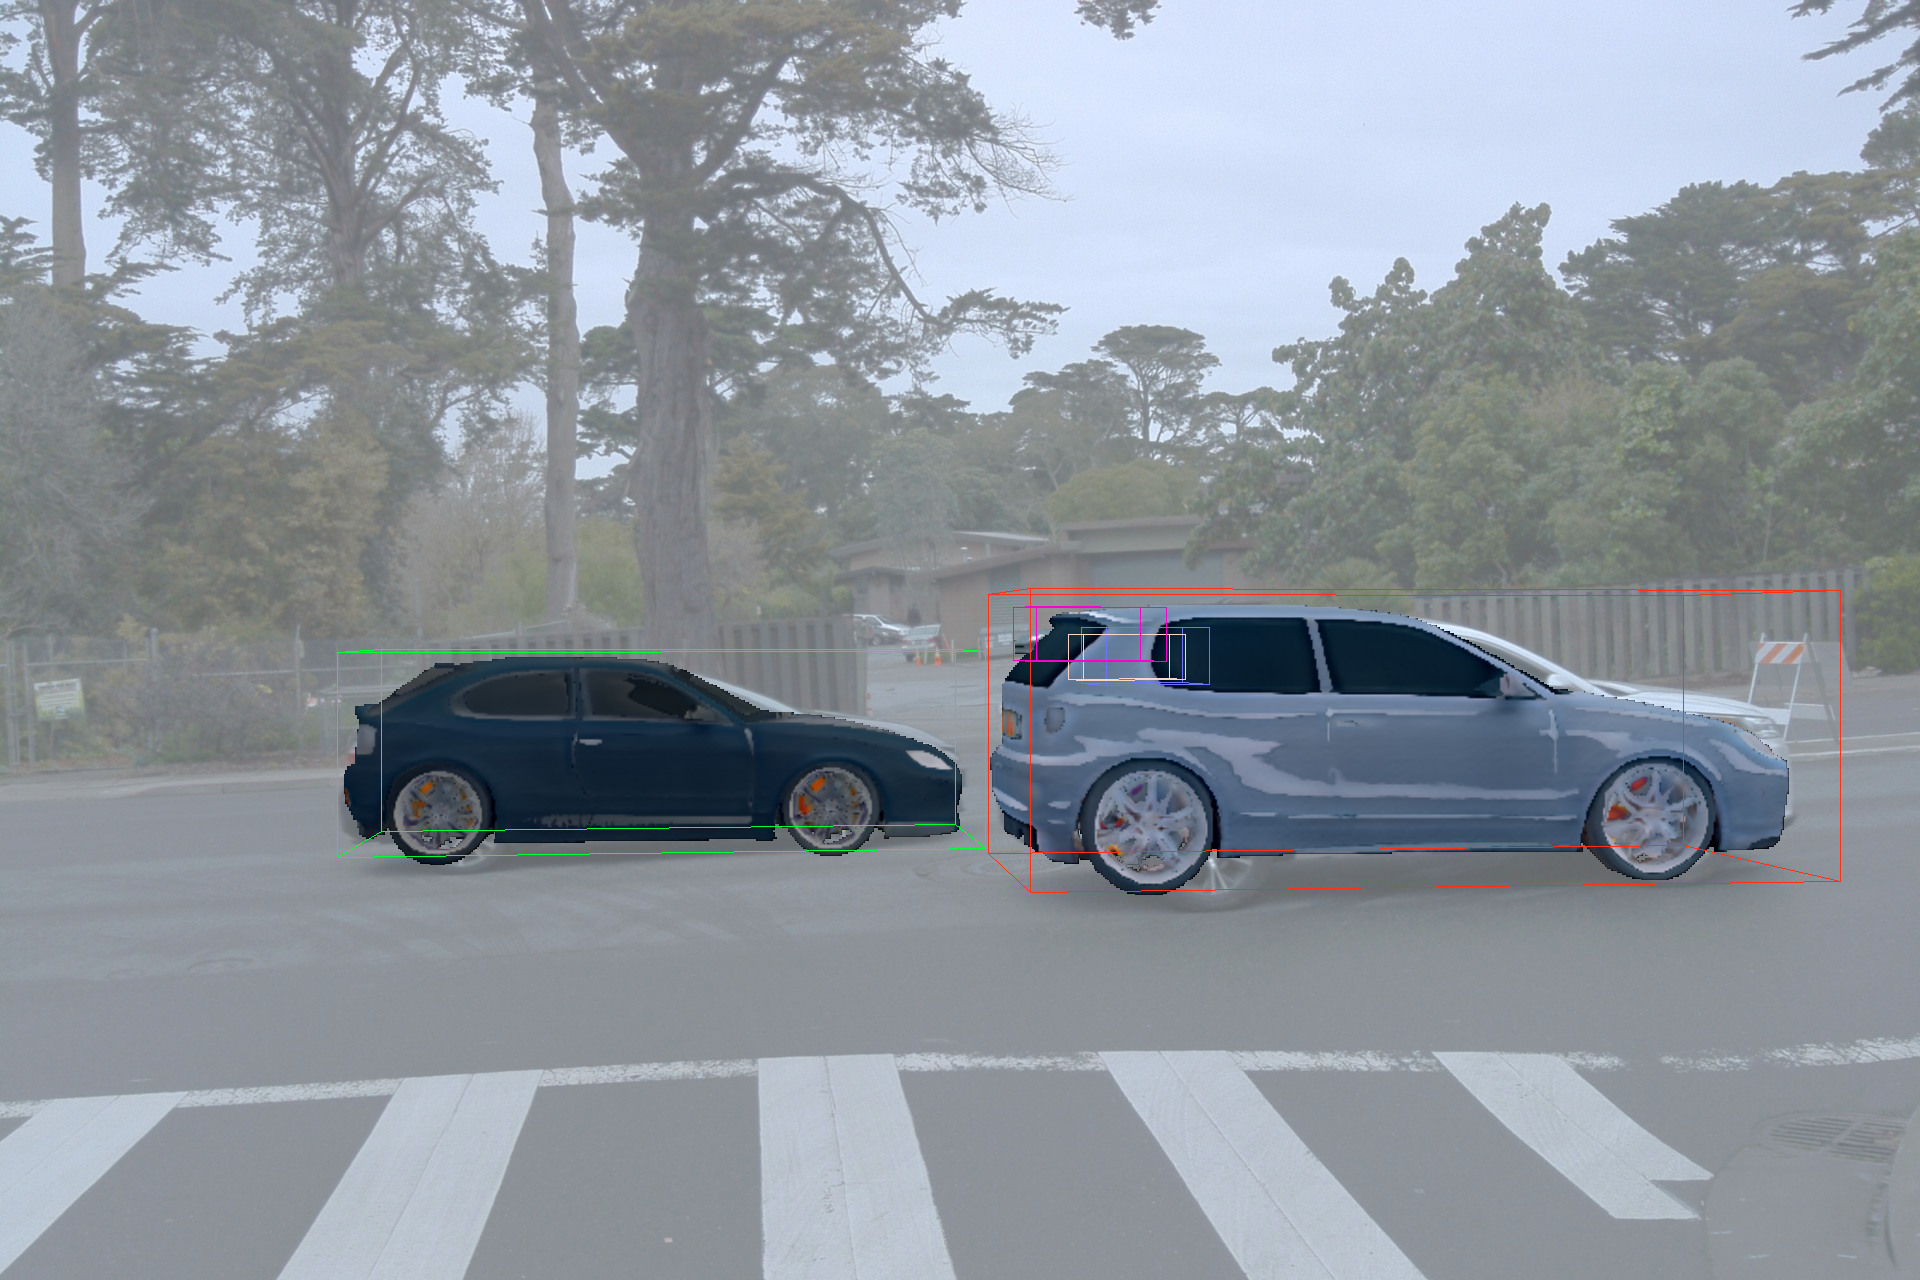
\includegraphics[width=.44\columnwidth, trim={0cm 0cm 0cm 0cm},clip]{fig/optim_supplement/scene11_104/5.png}





\end{tabular}}\vspace*{-6pt}
\caption{\textbf{Optimization Process.} From left to right, we show (i) the observed image, (ii) the rendering predicted by the initial starting point latent embeddings, 
(iii) the predicted rendered objects after the texture code is optimized (iv) the predicted rendered objects after the translation, scale, and rotation are optimized, and (v) the predicted rendered objects after the shape latent code is optimized. The ground truth images are faded to show our rendered objects clearly. Our method is capable of refining the predicted texture, pose, and shape over several optimization steps, even if initialized with poses or appearances far from the target -- all corrected through inverse rendering.}
\label{fig:optim}
\vspace{-8pt}
\end{figure*}